\documentclass[11pt,          % font size: 11pt or 12pt
               ms,           % degree:    ms or phd
               onehalfspacing,% spacing: onehalfspacing or doublespacing
               ]{ncsuthesis}

\usepackage[utf8]{inputenc}

%%----------------------------------------------------------------------------%%
%%------------------------------ Import Packages -----------------------------%%
%%----------------------------------------------------------------------------%%

\usepackage{booktabs}  % professionally typeset tables
\usepackage{amsmath}
\usepackage{textcomp}  % better copyright sign, among other things
\usepackage{xcolor}
\usepackage{lipsum}    % filler text
\usepackage{longtable}
%\usepackage{subfig}    % composite figures
%\usepackage{fancyhdr}  % creates headers
%\pagestyle{fancy}

% \usepackage{natbib}    % ability to use citet,citep

\usepackage[outdir=./hidden_epstopdf/]{epstopdf}

% setup bibliography
\usepackage[american]{babel} % periods inside quotations in citations
\usepackage{csquotes} % required by babel
\usepackage[
      %style=alphabetic,%
      style=numeric,%
      sorting=none,%nyt,ynt          
      hyperref=true, %  
      giveninits=true,%
      backend=biber,
      bibencoding=utf8,%
      natbib=true,
      url=false,
      isbn=false,
      maxnames=2, %for et al to be used
      maxalphanames=1, %to avoid printing a + for every et al in abbreviation
      doi=true,
      sortcites, % sort multicite events (multiple citations in one command)
]{biblatex}    
\addbibresource{WilliamDawn-thesis.bib}

%%----------------------------------------------------------------------------%%
%%---------------------------- Formatting Options ----------------------------%%
%%----------------------------------------------------------------------------%%
%%

%% -------------------------------------------------------------------------- %%
%% Disposition format -- any titles, headings, section titles
%%  These formatting commands affect all headings, titles, headings,
%%  so sizing commands should not be used here.
%%  Formatting options to consider are
%%     +  \sffamily - sans serif fonts.  Dispositions are often typeset in
%%                    sans serif, so this is a good option. 
%%     +  \rmfamily - serif fonts
%%     +  \bfseries - bold face
%\dispositionformat{\sffamily\bfseries}   % bold and sans serif
\dispositionformat{\bfseries}            % bold and serif

%% -------------------------------------------------------------------------- %%
%% Formatting for centered headings - Abstract, Dedication, etc. headings
%%  This is where one might put a sizing command.
%%  \MakeUppercase can be used to typeset all headings in uppercase.
\headingformat{\large\MakeUppercase}   % All letters uppercase
%\headingformat{\large}                % Not all uppercase
%\headingformat{\Large\scshape}        % Small Caps, used with serif fonts.

%% Typographers recommend using a normal inter-word space after
%% sentences. TeX's default is to add an wider space, but \frenchspacing
%% gives a normal spacing. Comment out the following line if you prefer wider spaces between sentences.
\frenchspacing

%% -------------------------------------------------------------------------- %%
%%  Optional packages
%%    A number of compatible packages to improve the look and feel of
%%    your document are available in the file optional.tex 
%%    (For example, hyperlinks, fancy chapter headings, and fonts)
%% To use these options, uncomment the next line and see optional.tex
\input{optional}
%solve bug from fancyhdr in optional
%http://nw360.blogspot.com/2006/11/latex-headheight-is-too-small.html
\setlength{\headheight}{26.94345pt} % corrected error in Overleaf
\fancyhead[L]{\vspace{1mm}} % only puts chapter title in headers

%%----------------------------------------------------------------------------%%
%%---------------------------- Content Options -------------------------------%%
%%----------------------------------------------------------------------------%%
%% Size of committee: 3, 4, 5, or 6 -- this number includes the chair
\committeesize{3}

%% Members of committee
%%  Each of the following member commands takes an optional argument
%%   to specify their role on the committee.
%%  For co-chairs, use the commands:
%%      \cochairI{Doug Dodd}
%%      \cochairII{Chris Cox}
%%
\chair{Scott P. Palmtag}
\memberI{Joseph M. Doster}
\memberII{Ralph C. Smith}
%\memberIII{Ralph C. Smith}   % unnecessary if committeesize=3
%\memberIV{Steven P. Hamilton}    % unnecessary if committeesize=3, 4

%% Student writing thesis, \student{First Middle}{Last}
\student{William Christopher}{Dawn} % a full middle name

%% Degree program e.g. Marine, Earth, and Atmospheric Science
\program{Nuclear Engineering}

%%!!!!!! To Change Year !!!!!!%%
% If year of graduation is not same as current year (common for December graduates
% thanks to the Grad Schools odd graduation rules) go into ncsuthesis.cls and change 
% \the\year in the line:
% \newcommand{\ncsu@year}{\the\year}
% to the year of graduation. E.g.:
\makeatletter
\renewcommand{\ncsu@year}{2019}
\makeatother

%% Thesis Title
%%  Keep in mind, according to ETD guidelines:
%%    +  Capitalize first letter of important words.
%%    +  Use inverted pyramid shape if title spans more than one line.
%%
%%  Note: To break the title onto multiple lines, use \break instead of \\.
%\thesistitle{A North Carolina State University Sample \LaTeX{} Thesis \break 
%with a Title So Long it Needs a Line Break}
\thesistitle{Simulation of Fast Reactors with the Finite Element Method and Multiphysics Models}

%% Degree year. Necessary if your degree year doesn't equal the current year.
%\degreeyear{1995}

%% While your here make sure to change the PDF characteristics in optional.tex!!!

%%----------------------------------------------------------------------------%%
%%---------------------------- Personal Macros -------------------------------%%
%%----------------------------------------------------------------------------%%

%% A central location to add your favorite macros.

\setacronymstyle{long-short}
\makeglossaries

\newacronym{fem}   {FEM}   {Finite Element Method}
\newacronym{spd}   {SPD}   {Symmetric Positive Definite}
\newacronym{sor}   {SOR}   {Successive Over-Relaxation}
\newacronym{cg}    {CG}    {Conjugate Gradient}
\newacronym{ebr-i} {EBR-I} {Experimental Breeder Reactor I}
\newacronym{ebr-ii}{EBR-II}{Experimental Breeder Reactor II}
\newacronym{vtr}   {VTR}   {Versatile Test Reactor}
\newacronym{inl}   {INL}   {Idaho National Laboratory}
\newacronym{sfr}   {SFR}   {Sodium-cooled Fast Reactor}
\newacronym{lwr}   {LWR}   {Light Water Reactor}
\newacronym{anl}   {ANL}   {Argonne National Laboratory}
\newacronym{geh}   {GEH}   {GE-Hitachi Nuclear Energy Americas LLC}
\newacronym{ulof}  {ULOF}  {Unprotected Loss-Of-Flow}
\newacronym{ulohs} {ULOHS} {Unprotected Loss-Of-Heat-Sink}
\newacronym{atws}  {ATWS}  {Anticipated Transient Without Scram}
\newacronym{lef}   {LEF}   {Linear Expansion Factor}
\newacronym{oecd}  {OECD}  {Organisation for Economic Co-operation and Development}
\newacronym{nea}   {NEA}   {Nuclear Energy Energy}
\newacronym{abr}   {ABR}   {Advanced Burner Reactor}
\newacronym{pcm}   {pcm}   {percent-mille ($10^{-5}$)}
\newacronym{ctc}   {CTC}   {Coolant Temperature Coefficient}
\newacronym{mtc}   {MTC}   {Moderator Temperature Coefficient}
\newacronym{cram}  {CRAM}  {Chebyshev Rational Approximation Method}
\newacronym{hwr}   {HWR}   {Heavy Water Reactor}
\newacronym{pwr}   {PWR}   {Pressurized Water Reactor}
\newacronym{fbr}   {FBR}   {Fast Breeder Reactor}
\newacronym{ornl}  {ORNL}  {Oak Ridge National Laboratory}
\newacronym{casl}  {CASL}  {Consortium for Advanced Simulation of LWRs}
\newacronym{iup}   {IUP}   {Integrated University Program}
\newacronym{doe-ne}{DOE-NE}{U.S. Department of Energy Office of Nuclear Energy}
\newacronym{spn}   {S$P_N$}{Simplified $P_N$}
\newacronym{rcm}   {RCM}   {Reverse Cuthill-McKee}
\newacronym{rms}   {RMS}   {Root-Mean-Squared}

\usepackage[section, above, below]{placeins}
% above & below helps to relax the strict FloatBarrier
% this helps in the thermal conductivities appendix

%\usepackage{draftwatermark}

\usepackage{xcolor}

\usepackage{sectsty}
\allsectionsfont{\raggedright}

\usepackage[chapter]{algorithm} % make sure to reset count at the new chapter
\usepackage[noend]{algpseudocode}
\renewcommand{\thealgorithm}{\arabic{chapter}.\arabic{algorithm}}

\usepackage{csvsimple}

\usepackage{subcaption}
\usepackage{threeparttable}

\usepackage{isotope}

\usepackage{float}

% reduce line spacing in verbatim environment to make things look more reasonable
% 1.0 would be a more reasonable value but 0.0 looks good for ascii art
\makeatletter
\def\verbatim@font{\linespread{0.0}\normalfont\ttfamily}
\makeatother

\usepackage[all]{nowidow}

\usepackage{textcomp} % texttrademark

% define a command called \titlebreak that will only break in the text, not table of contents
% table of contents needs to be wrapped like
% \begingroup\intoctrue
% \tableofcontents
% \endgroup
\newif\ifintoc
\DeclareRobustCommand{\titlebreak}{%
  \ifintoc
    \unskip\space
  \else
    \newline
  \fi
}

\renewcommand{\epsilon}{\varepsilon}

\newenvironment{conditions}{\par\noindent\begin{tabular}{l@{${}={}$}l}}{\end{tabular}\vspace{0.25\baselineskip}\par\noindent}

\usepackage{footnote}
\makesavenoteenv{tabular} % allow footnotes at bottom of page for a table
\makesavenoteenv{figure} % allow footnotes at bottom of page for a table
\renewcommand*{\thefootnote}{\fnsymbol{footnote}} % use symbols instead of numbers in footnotes

\usepackage{siunitx}
\DeclareSIUnit{\dof}{\glsentryshort{dof}}
\DeclareSIUnit{\pcm}{\glsentryshort{pcm}}
\DeclareSIUnit{\mfp}{\glsentryshort{mfp}}
\DeclareSIUnit{\weightpercent}{wt.\!\unit{\percent}}
\DeclareSIPrefix{\million}{M}{6}
\DeclareSIPrefix{\billion}{B}{9}

\usepackage{makecell} % thead
\usepackage{textcomp}

\newcommand{\mc}[1]{\multicolumn{1}{c}{#1}}

\usepackage{tikz}
\usepackage{varwidth, enumitem}
\usetikzlibrary{decorations.pathreplacing}
\usetikzlibrary{calc}
\usetikzlibrary{shapes, arrows.meta, positioning}

%%%% % save tikz images to pdfs
%%%% \usetikzlibrary{external}
%%%% \tikzexternalize % activate!

% segment length      -- distance between waves
% amplitude           -- width of waves
% meta-segment length -- degree of waviness
\pgfdeclaredecoration{discontinuity}{start}{
  \state{start}[width=0.5\pgfdecoratedinputsegmentremainingdistance-0.5\pgfdecorationsegmentlength,next state=first wave]
  {}
  \state{first wave}[width=\pgfdecorationsegmentlength, next state=second wave]
  {
    \pgfpathlineto{\pgfpointorigin}
    \pgfpathmoveto{\pgfqpoint{0pt}{\pgfdecorationsegmentamplitude}}
    \pgfpathcurveto
        {\pgfpoint{-0.25*\pgfmetadecorationsegmentlength}{0.75\pgfdecorationsegmentamplitude}}
        {\pgfpoint{-0.25*\pgfmetadecorationsegmentlength}{0.25\pgfdecorationsegmentamplitude}}
        {\pgfpoint{0pt}{0pt}}
    \pgfpathcurveto
        {\pgfpoint{0.25*\pgfmetadecorationsegmentlength}{-0.25\pgfdecorationsegmentamplitude}}
        {\pgfpoint{0.25*\pgfmetadecorationsegmentlength}{-0.75\pgfdecorationsegmentamplitude}}
        {\pgfpoint{0pt}{-\pgfdecorationsegmentamplitude}}
}
\state{second wave}[width=0pt, next state=do nothing]
  {
    \pgfpathmoveto{\pgfqpoint{0pt}{\pgfdecorationsegmentamplitude}}
    \pgfpathcurveto
        {\pgfpoint{-0.25*\pgfmetadecorationsegmentlength}{0.75\pgfdecorationsegmentamplitude}}
        {\pgfpoint{-0.25*\pgfmetadecorationsegmentlength}{0.25\pgfdecorationsegmentamplitude}}
        {\pgfpoint{0pt}{0pt}}
    \pgfpathcurveto
        {\pgfpoint{0.25*\pgfmetadecorationsegmentlength}{-0.25\pgfdecorationsegmentamplitude}}
        {\pgfpoint{0.25*\pgfmetadecorationsegmentlength}{-0.75\pgfdecorationsegmentamplitude}}
        {\pgfpoint{0pt}{-\pgfdecorationsegmentamplitude}}
    \pgfpathmoveto{\pgfpointorigin}
}
  \state{do nothing}[width=\pgfdecorationsegmentlength,next state=do nothing]{
    \pgfpathlineto{\pgfpointdecoratedinputsegmentlast}
  }
  \state{final}
  {
    \pgfpathlineto{\pgfpointdecoratedpathlast}
  }
}

\graphicspath{
  {./ch01_introduction/figs/}
  {./ch02_neutronDiffusion/figs/}
  {./ch03_diffusionResults/figs/}
  {./ch04_thermalHydraulics/figs/}
  {./ch05_thermalExpansion/figs/}
  {./ch06_coupledResults/figs/}
  {./ch07_conclusions/figs/}
  {./apA_analyticSolutions/figs/}
  {./apB_benchmarks/figs/}
  }

\usepackage{xspace}

% linear algebra
\renewcommand{\epsilon}{\varepsilon} % use the pretty epsilon

%    vectors
\newcommand{\va}{\mathbf{a}}
\newcommand{\vb}{\mathbf{b}}
\newcommand{\vc}{\mathbf{c}}
\newcommand{\vd}{\mathbf{d}}
\newcommand{\ve}{\mathbf{e}}
\newcommand{\vf}{\mathbf{f}}
\newcommand{\vp}{\mathbf{p}}
\newcommand{\vr}{\mathbf{r}}
\newcommand{\vu}{\mathbf{u}}
\newcommand{\vx}{\mathbf{x}}
\newcommand{\vw}{\mathbf{w}}
\newcommand{\vPhi}{\Phi}

%    matrices
\newcommand{\ma}{\mathbf{A}}
\newcommand{\mb}{\mathbf{B}}
\newcommand{\mj}{\mathbf{J}}
\newcommand{\ml}{\mathbf{L}}
\newcommand{\mm}{\mathbf{M}}
\newcommand{\mr}{\mathbf{R}}

%    sets
\newcommand{\real}{\mathbb{R}}
\newcommand{\realn}{\real^{n}}
\newcommand{\realnn}{\real^{n \times n}}

% variable definitions
\newcommand{\keff}{\ensuremath{k_{\!\mbox{\scriptsize \em eff}}}\xspace}
\newcommand{\keffsub}[1]{\ensuremath{k_{\!\mbox{\scriptsize \em eff,{#1}}}}}
\newcommand{\kref}{\ensuremath{k_{\!\mbox{\scriptsize \em ref}}}}
\newcommand{\grad}{\mathbf{\nabla}}

% neutronDiffusion
\newcommand{\albedo}{\alpha}
\newcommand{\basis}{N}
\newcommand{\twotable}{TwoTable }
\newcommand{\phiavg}{\overline{\phi}}
\newcommand{\nhat}{\hat{\mathbf{n}}}

% diffusionResults
\newcommand{\true}{\checkmark}

% code names
\newcommand{\dif}{\text{DIF3D}\xspace}
\newcommand{\mcc}{\text{MC**2}\xspace}

% thermalHydraulics
\newcommand{\mdot}{\dot{m}}

% thermalExpansion
\newcommand{\texpfuel}
  {\ensuremath{{T_{\!\mbox{\scriptsize \em fuel}}}}}
\newcommand{\texpstruct}
  {\ensuremath{T_{\!\mbox{\scriptsize \em struct}}}}

% general macros
\newcommand{\units}[1]{\ensuremath{\left[\text{{#1}}\right]}}
\newcommand{\half}{\frac{1}{2}}
\newcommand{\nicesub}[2]{\ensuremath{{#1}_{\!\mbox{\scriptsize \em {#2}}}}}

% reference macros
\newcommand{\eref}[1]{Eq.~(\ref{#1})}
\newcommand{\fref}[1]{Fig.~\ref{#1}}
\newcommand{\tref}[1]{Table~\ref{#1}}
\newcommand{\sref}[1]{\S\ref{#1}}
\newcommand{\chref}[1]{Chapter~\ref{#1}}
\newcommand{\apref}[1]{Appendix~\ref{#1}}
\newcommand{\algorithmref}[1]{Algorithm~\ref{#1}}

\usepackage{array}
\newcolumntype{L}{>{$}l<{$}}
% \newenvironment{conditions}
%   {\par\vspace{\abovedisplayskip}\noindent\begin{tabular}{>{$}l<{$} @{${}={}$} l}}
%   {\end{tabular}\par\vspace{\belowdisplayskip}}
\newenvironment{conditions}
  {\par\noindent\begin{tabular}{L @{${}={}$} l}}{\end{tabular}\par}


\usepackage{calc}
%% Capital letter height
\newlength{\chaptercapitalheight}
\settoheight{\chaptercapitalheight}{D}
\newlength{\chapterfootskip}
\setlength{\chapterfootskip}{\chaptercapitalheight}
\addtolength{\chapterfootskip}{2\baselineskip}

%landscape support in fancyhdr from 
%http://tex.stackexchange.com/questions/9071/how-to-translate-and-rotate-the-heading-of-landscaped-pages
\usepackage{pdflscape}
\usepackage{tikz}
\fancypagestyle{lscapedplain}{%
  \fancyhf{}
  \fancyfoot{%
    \tikz[remember picture,overlay]
      \node[outer sep=1cm,above,rotate=90] at (current page.east) {\thepage};}
\renewcommand{\headrulewidth}{0pt} 
\renewcommand{\footrulewidth}{0pt}
}

%%---------------------------------------------------------------------------%%
\begin{document}
%%---------------------------------------------------------------------------%%
\frontmatter

%% ------------------------------ Abstract ---------------------------------- %%
\begin{abstract}
  \lipsum[1-6]
\end{abstract}

%% ---------------------------- Copyright page ------------------------------ %%
\makecopyrightpage

%% -------------------------------- Title page ------------------------------ %%
\maketitlepage

%% -------------------------------- Dedication ------------------------------ %%
\begin{dedication}
  \centering To the future of clean energy.
\end{dedication}

%% -------------------------------- Biography ------------------------------- %%
\begin{biography}
  The author was born in a small town \ldots
\end{biography}

%% ----------------------------- Acknowledgements --------------------------- %%
\begin{acknowledgements}
  I would like to thank my advisor for his help.
\end{acknowledgements}

\thesistableofcontents

\thesislistoftables

\thesislistoffigures


%%---------------------------------------------------------------------------%%
\mainmatter

\chapter{Introduction}
\label{ch:introduction}

\section{Motivation}
\section{Geometry Description}
  \label{sec:geometry_description}
  % include can figure

  \begin{figure}
    \centering
    \includegraphics[width=\textwidth]{reactor_materials}
    \caption{Example of Sodium-cooled Fast Reactor based on MONJU.}
    \label{fig:reactor_materials}
  \end{figure}

  In a cross-sectional assembly view, dimensions are presented in
  \fref{fig:pin_model} and \fref{fig:hex_can}. In \fref{fig:hex_can}, $Th_{Box}$
  is the thickness of the assembly box, F2F is the flat-to-flat measurement of
  the outside of the hexagonal can, and Pitch is the distance between the
  center of two pins. In future notation, the quantity ``Pitch'' is also denoted
  $S$. Using the geometry described in these figures, the material
  cross-sectional areas are calculated according to the given formulae where
  $N_{pin}$ is the number of pins in the assembly.
  \begin{align}
    \label{eq:afrac_first}
    A_{total} &= \frac{\sqrt{3}}{2} F2F^2 \\
    A_{can} &= A_{total} - 
      \frac{\sqrt{3}}{2} \left(  F2F - 2 \, Th_{Box} \right) \\
    A_{wrap} &= N_{pin} \frac{\pi}{4} D_{wrap}^2 \\
    A_{clad} &= N_{pin} \pi (R_C^2 - R_B^2) \\
    A_{bond} &= N_{pin} \pi (R_B^2 - R_F^2) \\
    A_{fuel} &= N_{pin} \pi R_F^2 \\
    \label{eq:afrac_last}
    A_{cool} &= A_{total} - A_{can} - A_{wrap} - A_{clad} - A_{bond} - A_{fuel}
  \end{align}
  Calculating the areas as above allows for calculation of cross-sectional area
  fractions. Assuming constant dimensions within an element in the axial
  direction, these area fractions are equivalent to volume fractions and are
  useful for neutron cross-section calculations. Additionally, these formulae
  allow for thermal expansion calculations as the liquid sodium in the bond and
  the coolant are allowed to vary to allow for the expansion of other materials.

  \begin{figure}
    \centering
    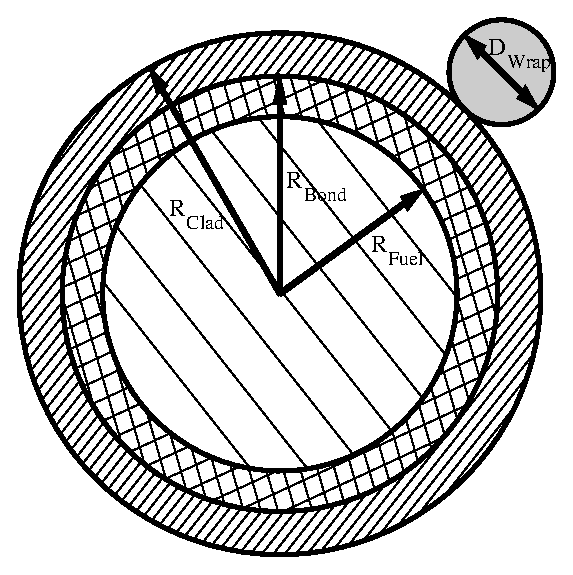
\includegraphics[width=0.5\textwidth]{pin_model}
    \caption{Dimensions of Thermal Hydraulic Pin Model.}
    \label{fig:pin_model}
  \end{figure}

  \begin{figure}
    \centering
    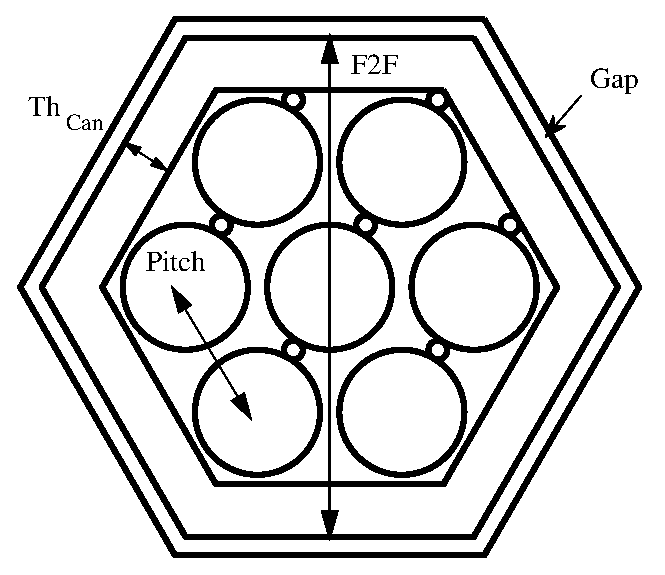
\includegraphics[width=0.5\textwidth]{hex_can}
    \caption{Dimensions of Hexagonal Can.}
    \label{fig:hex_can}
  \end{figure}

\section{Cross Section Generation}

\chapter{FINITE ELEMENT NEUTRON DIFFUSION}
\label{ch:neutronDiffusion}

\section{Introduction}
  For typical nuclear reactor applications, diffusion theory well approximates 
  the neutron distribution within the reactor. The neutron diffusion equation is
  a second order partial differential equation in space and energy. In standard
  notation, the continuous neutron diffusion equation is presented as
  \begin{multline}\label{eq:continuous_diffusion}
    -\grad \cdot (D(\vr,E) \grad \phi(\vr,E)) + \Sigma_t(\vr,E) \phi(\vr,E) = \\
      \frac{\chi(\vr,E)}{\keff} \int_0^{\infty} \nu_f(\vr,E') \Sigma_f(\vr,E') 
      \phi(\vr,E') \; dE' + \int_0^{\infty} \Sigma_s(\vr,E' \rightarrow E) 
      \phi(\vr,E') \; dE'
  \end{multline}
  Where $D$ is the diffusion constant, $\phi$ is the scalar neutron flux, 
  $\Sigma_t$ is the total cross section, $\chi$ is the fission neutron 
  spectrum, $\keff$ is the effective neutron multiplication factor, $\Sigma_f$ 
  is the fission cross section, $\nu_f$ is the neutron yield per fission, and 
  $\Sigma_s(\vr,E' \rightarrow E)$ is the scattering cross section for neutrons 
  at position $\vr$ scattering from energy $E'$ to $E$.
  
  The neutron diffusion equation must be discretized in space and 
  energy to be solved numerically. Energy discretization is relatively 
  straight-forward and is performed using the multigroup method. Spatial 
  discretization requires more attention and will be done with the Finite 
  Element Method (FEM). This method is selected for several reasons. It allows
  for easily increasing the order of the method by increasing the order of the 
  elements with no changing of the mesh required. Coordinates of nodes can be 
  easily updated to reflect physical phenomena such as thermal expansion 
  (\chref{ch:thermalExpansion}). Additionally, material properties are 
  calculated on an element basis allowing for fine detail updates to the 
  material properties during the calculation.
  
  For energy discretization, An energy structure is described as $\{E_g\}$ for 
  $g = 1,2,\ldots,G$ and by convention
  \[ E_G > E_{G-1} > \ldots > E_2 > E_1  \]
  Then, multigroup constants can be calculated based on the energy group 
  structure and the known cross sections. Multigroup constants are calculated to
  preserve the number of neutrons produced or destroyed. That is, the 
  calculation preserves reaction rates where the reaction rate for reaction $x$
  is defined as $R_x=\Sigma_x \phi$. Multigroup constants are then calculated. A
  formal derivation is given in \cite{duderstathamilton} and the results are 
  presented below.
  \begin{align}
    D_g(\vr) &= \frac{\int_{E_g}^{E_{g-1}} D(\vr,E') \grad \phi(\vr,E)\;dE}
      {\int_{E_g}^{E_{g-1}} \grad \phi(\vr,E)\;dE} \\
    \Sigma_{t,g}(\vr) &= \frac{\int_{E_g}^{E_{g-1}} \Sigma_t(\vr,E) 
      \phi(\vr,E)\;dE}{\int_{E_g}^{E_{g-1}} \phi(\vr,E)\;dE} \\
    \nu\Sigma_{f,g}(\vr) &= \frac{\int_{E_g}^{E_{g-1}} \nu_f(\vr,E)
      \Sigma_f(\vr,E) \phi(\vr,E)\;dE}{\int_{E_g}^{E_{g-1}} 
      \phi(\vr,E)\;dE} \\
    \Sigma_{s,g\rightarrow g'}(\vr) &= \frac{\int_{E_g'}^{E_{g'-1}} 
      \int_{E_g}^{E_{g-1}} \Sigma_s(\vr,E' \rightarrow E) \phi(\vr,E')\;dE\;dE'}
      {\int_{E_g}^{E_{g-1}} \phi(\vr,E)\;dE}  \\
    \chi_g(\vr) &= \int_{E_g}^{E_{g-1}} \chi(\vr,E) \; dE \\
    \phi_g(\vr) &= \int_{E_g}^{E_{g-1}} \phi(\vr,E) \; dE
  \end{align}
  Note that cross sections $\nu_f(\vr,E)$ and $\Sigma_f(\vr,E)$ have been 
  combined. This is necessary and a mathematical result of the group collapse.
  Then, \eref{eq:continuous_diffusion} can be discretized in energy as
  \begin{align}\label{eq:multigroup_diffusion}
    - \grad \cdot ( D_g(\vr) \grad \phi_g(\vr)) + \Sigma_{t,g}(\vr) \phi_g(\vr)= 
      \frac{\chi_g(\vr)}{\keff} \sum_{g'=1}^{G} \nu\Sigma_{f,g'}(\vr) 
      \phi_{g'}(\vr) + \sum_{g'=1}^{G} \Sigma_{s,g' \rightarrow g}(\vr) 
      \phi_{g'}(\vr)
  \end{align}
  The neutron diffusion equation has now been discretized in energy.
  Spatial dicretization will be based on the Finite Element Method (FEM) and 
  will be discussed in \sref{sec:formulation:derivation}.
  
  % todo this discussion may need to be moved to 'Implementation'
  The total neutron cross section includes the contribution due to 
  self-scattering. That is, due to $\Sigma_{s,g\rightarrow g}$. This can be 
  removed from \eref{eq:multigroup_diffusion} for simplicity.
  \begin{equation} \label{eq:multigroup_removal}
    - \grad \cdot( D_g(\vr) \grad \phi_g(\vr)) + \Sigma_{r,g}(\vr) \phi_g(\vr) = 
      \frac{\chi_g(\vr)}{\keff} \sum_{g'=1}^{G} \nu\Sigma_{f,g'}(\vr) 
      \phi_{g'}(\vr) + \sum_{g'=1, g' \ne g}^{G} \Sigma_{s,g' \rightarrow g}(\vr) 
      \phi_{g'}(\vr)
  \end{equation}
  Where $\Sigma_{r,g}$ is the removal cross section and $\Sigma_{r,g}(\vr) = 
  \Sigma_{t,g}(\vr) - \Sigma_{s,g\rightarrow g}(\vr)$. For simplicity, the
  neutron sources in \eref{eq:multigroup_removal} can be  combined into a
  single term.
  \begin{equation} \label{eq:multigroup_source}
    - \grad \cdot( D_g(\vr) \grad \phi_g(\vr)) + \Sigma_{r,g}(\vr) \phi_g(\vr) = 
      q_g(\vr)
  \end{equation}
  Where $q_g(\vr)$ is the combined neutron source at position $\vr$. $q$ can 
  then be further divided into contributions due to fission ($q_{fiss}$), up-
  scattering ($q_{up}$) when a neutron increases in energy, and down-scattering 
  when a neutron decreases in energy ($q_{down}$).
  \begin{align}
    q_g(\vr) &= q_{fiss,g}(\vr) + q_{up,g}(\vr) + q_{down,g}(\vr) \\
    q_{fiss,g}(\vr) &= \frac{\chi_g(\vr)}{\keff} \sum_{g'=1}^{G} 
      \nu \Sigma_{f,g'}(\vr) \phi_{g'}(\vr) \\
    q_{up,g}(\vr) &= \sum_{g'=g+1}^{G} \Sigma_{s,g' \rightarrow g}(\vr)
      \phi_{g'}(\vr) \\
    q_{down,g}(\vr) &= \sum_{g'=1}^{g} \Sigma_{s,g' \rightarrow g}(\vr)
      \phi_{g'}(\vr)
  \end{align}
  Where the difference between $q_{up}$ and $q_{down}$ are the limits of the 
  summation. This form allows for operator splitting of the neutron source term.
  In an iterative scheme, it will be necessary for fission and up-scatter 
  sources to use a different flux iterate than down-scatter so this division
  will prove useful.
  

\section{Formulation}
  \subsection{Derivation}
    \label{sec:formulation:derivation}
    The only remaining continuous variable in the problem is the spatial 
    variable $\vr$. This will be discretized according to the Finite Element 
    Method (FEM). The form of the diffusion equation to be discretized is 
    \eref{eq:multigroup_source}. The problem is solved in a finite domain 
    $\vr \in \Omega$ where $\partial \Omega$ represents the boundary of the 
    domain where some boundary condition is specified. Boundary condition 
    options provided include
    \begin{enumerate}
      \item Mirror. $\grad \phi_g(\vr) = 0$ for $\vr \in \partial \Omega$.
      \item Albedo. $D_g(\vr) \grad \phi_g(\vr) + \albedo \phi_g(\vr)=0$ for 
        $\vr \in \partial \Omega$ where $\albedo$ is a real constant specified
        by the user. For vacuum conditions, $\alpha = \half$.
      \item Zero Flux. $\phi_g(\vr) = 0$ for $\vr \in \partial \Omega$.
    \end{enumerate}
    (Note: the order of the above list corresponds to the order of boundary 
    condition precedent in code with the greater the integer, the greater the 
    precedent.)
    
    Finite Element derivation begins with \eref{eq:multigroup_source}.
    The equation is multiplied by a testing function $v(\vr) \in H_1(\Omega)$ 
    Where $H$ is the Sobolev Space. Then, the equation is integrated over the 
    problem domain. This yields the Weak Form or Variational Form of the 
    problem.
    \begin{align}
      -\grad \cdot (D_g(\vr) \grad \phi_g(\vr)) + \Sigma_{r,g}(\vr) \phi_g(\vr)
        &=q_g(\vr) \\
      -\grad \cdot (D_g(\vr) \grad \phi_g(\vr)) v(\vr) + 
        \Sigma_{r,g}(\vr) \phi_g(\vr) v(\vr) &=
        q_g(\vr) \\
      - \int_{\Omega} \grad \cdot (D_g(\vr) \grad \phi_g(\vr)) v(\vr) \; d\Omega
        \int_{\Omega} \Sigma_{r,g}(\vr) \phi_g(\vr) v(\vr) \;d\Omega &=
        \int_{\Omega} q_g(\vr) v(\vr) \;d\Omega
    \end{align}
    
    For the purposes of this application, material cross sections and the
    neutron source are assumed to be constant within an element. Then, the 
    integral can be partitioned into a sum of integrals over the elements in the
    domain assuming the set of elements $\{\Omega_e\} = \Omega$ for 
    $e = 1,2,\ldots,E$ where $E$ is the total number of elements.
    \begin{equation} \label{eq:element_by_element}
      -\sum_{e=1}^{E} D_{g,e} 
        \int_{\Omega_e} \grad \cdot \grad \phi_g(\vr) v(\vr) \; d\Omega_e +
        \sum_{e=1}^{E} \Sigma_{r,g,e} \int_{\Omega_e} \phi_g(\vr) v(\vr) 
        \;d\Omega_e = \sum_{e=1}^{E} q_{g,e} \int_{\Omega_e} v(\vr) 
        \; d\Omega_e
    \end{equation}
    The Second Green's Theorem is used to simplify the integral in the first
    term. A proof can be found in \cite{textbookli} in Theorem 9.2.
    \begin{equation} \label{eq:greens}
      -\int_{\Omega_e} \grad \cdot \grad \phi_g(\vr) v(\vr) \;d\Omega_e =
        -\int_{\partial \Omega_e}  
        \frac{\partial \phi_g(\vr)}{\partial \vn} v(\vr)\; ds + \int_{\Omega_e} 
        \grad \phi_g(\vr) \cdot \grad v(\vr) \; d\Omega_e
    \end{equation}
    Where $\frac{\partial \phi_g(\vr)}{\partial \vn}$ is the outward normal 
    derivative and the integral $ds$ is a line integral in two dimensions or a 
    surface integral in three dimensions. Recognizing that this quantity will 
    only be relevant on the boundary of the problem, the value of the outward 
    normal derivative may be specified in a boundary condition. Specifically, 
    the Albedo boundary condition which has the following form for $\vr \in 
    \partial \Omega$. 
    \begin{align}
      D_g(\vr) \grad \phi_g(\vr) + \albedo \phi_g(\vr) &= 0 \\
      \grad \phi_g(\vr) &= \frac{-\albedo \phi_g(\vr)}{D_g}
    \end{align}
    Substituting \eref{eq:greens} into  \eref{eq:element_by_element} and 
    assuming the outward normal derivative is specified in the form of an Albedo
    boundary condition.
    \begin{multline} 
      -\sum_{e=1}^{E} D_{g,e} \int_{\partial \Omega_e} v(\vr) 
        \frac{\partial \phi_g(\vr)}{\partial \vn} \;ds + \sum_{e=1}^{E} D_{g,e}
        \int_{\Omega_e} \grad \phi_g(\vr) \cdot \grad v(\vr) \; d\Omega_e + \\
        \sum_{e=1}^{E} \Sigma_{r,g,e} \int_{\Omega_e} \phi_g(\vr) v(\vr) 
        \; d\Omega_e =
        \sum_{e=1}^{E} q_{g,e} \int_{\Omega_e} v(\vr) \; d\Omega_e
    \end{multline}
    \begin{multline} \label{eq:element_boundary}
      \sum_{e=1}^{E} \albedo \int_{\partial \Omega_e} v(\vr) 
        \phi_g(\vr) \;ds + \sum_{e=1}^{E} D_{g,e}
        \int_{\Omega_e} \grad \phi_g(\vr) \cdot \grad v(\vr) \; d\Omega_e + \\
        \sum_{e=1}^{E} \Sigma_{r,g,e} \int_{\Omega_e} \phi_g(\vr) v(\vr) 
        \; d\Omega_e =
        \sum_{e=1}^{E} q_{g,e} \int_{\Omega_e} v(\vr) \; d\Omega_e
    \end{multline}
    Now the function of interest $\phi_g(\vr)$ is assumed to be a linear 
    combination of chosen basis functions $\{\basis_i\}$.
    \begin{equation} \label{eq:linear_combination}
      \phi_g(\vr) = \sum_{i=1}^{N} \alpha_{g,i} \basis_i(\vr)
    \end{equation}
    Where coefficients $\{\alpha_i\}$ are unknown and will be determined. 
    Typically, these basis functions have unit magnitude and are centered at the
    node  points so the coefficients $\alpha_i$ are the approximated solution at
    the nodes. Basis functions are typically polynomials of arbitrary magnitude. 
    Linear and quadratic polynomials are common but for the application 
    presented here, only linear basis functions are explored.
    The test function $v(\vr)$ is also chosen as a linear combination of the 
    basis functions.
    \begin{equation} \label{eq:linear_superposition}
      v(\vr) = \sum_{j=1}^{N} \basis_j(\vr)
    \end{equation}
    The testing function is arbitrary so the magnitude is fixed to the magnitude
    of the basis function.
    
    \eref{eq:linear_combination} and \eref{eq:linear_superposition} are plugged
    into \eref{eq:element_boundary}. This yields a linear system of equations.
    \begin{multline}
      \sum_{e=1}^{E} \albedo \sum_{i=1}^{N} \alpha_{i,g}
        \int_{\partial \Omega_e}
        \basis_i(\vr)  \basis_j(\vr) \;ds +
        \sum_{e=1}^{E} D_{g,e} \sum_{i=1}^{N} \alpha_{i,g}
        \int_{\Omega_e} \grad \basis_i(\vr) \cdot \grad \basis_i(\vr)\;d\Omega_e
        + \\
        \sum_{e=1}^{E} \Sigma_{r,g,e} \sum_{i=1}^{N} \alpha_{i,g}
        \int_{\Omega_e} \basis_i(\vr) \basis_i(\vr) \; d\Omega_e =
        \sum_{e=1}^{E} q_{g,e} \sum_{i=1}^{N} 
        \int_{\Omega_e} \basis_i(\vr) \; d\Omega_e
    \end{multline}
    \begin{multline}
      \sum_{i=1}^{N} \alpha_{i,g} \sum_{j=1}^{N} \left(
        \sum_{e=1}^{E} \albedo \int_{\partial \Omega_e}
        \basis_i(\vr)  \basis_j(\vr) \;ds +
        \sum_{e=1}^{E} D_{g,e} 
        \int_{\Omega_e} \grad \basis_i(\vr) \cdot \grad \basis_j(\vr)\;d\Omega_e
        \right.
        + \\
        \left.
        \sum_{e=1}^{E} \Sigma_{r,g,e}
        \int_{\Omega_e} \basis_i(\vr) \basis_j(\vr) \; d\Omega_e \right) =
        \sum_{i=1}^{N} \left(
        \sum_{e=1}^{E} q_{g,e} 
        \int_{\Omega_e} \basis_i(\vr) \; d\Omega_e \right)
    \end{multline}
    \begin{align}
      \label{eq:fem_notation}
      a(\basis_i,\basis_j) &= f(\basis_i) \\
      \ma \vu &= \vf
    \end{align}
    $a(\basis_i,\basis_j)$ is the bilinear form and $f(\basis_i)$ is the linear 
    form of the finite element system. The notation of \eref{eq:fem_notation} is
    common to mathematical discussions of the FEM. The diffusion coefficient 
    $D_g(\vr)$ is nonzero and bounded and the removal cross section 
    $\Sigma_{r,g}(\vr)$ is bounded. Theorem 9.3 \cite{textbookli} then shows 
    that the finite element equations satisfy the Lax-Milgram Lemma implying 
    the solution to the finite element method are unique and bounded. This is 
    not purely the case as the source function $q_g(\vr)$ is updated on each 
    iteration. In each iteration a unique solution exists. The global problem
    remains an eigenvalue problem as described in \cite{duderstathamilton}. The
    method will return the fundamental eigenvalue $\keff$ and the shape function
    which must be normalized by an arbitrary constant.
    
    In matrix notation, $\ma$ is described by the integral quantities (more to 
    follow),  $\vu = \{\alpha_i\}$, and $\vf$ is described by the source 
    integral quantity. Inspecting the matrix $\ma$ and the vector $\vf$ reveals 
    the following.
    \begin{align}
      \label{eq:matrix_population}
      A_{i,j,g,e} &= \albedo \int_{\partial \Omega_e} \basis_i(\vr) 
        \basis_j(\vr) \; ds + D_{g,e} 
        \int_{\Omega_e} \grad \basis_i(\vr) \cdot \grad \basis_j(\vr) \;
        d\Omega_e + \Sigma_{r,g,e} \int_{\Omega_e} \basis_i(\vr) \basis_j(\vr)
        \; d\Omega_e \\
      \label{eq:vector_population}
      f_{i,g,e} &= q_{g,e} \int_{\Omega_e} \basis_i(\vr) \;d\Omega_e
    \end{align}
    Then, 
    \begin{align}
      A_{i,j,g} &= \sum_{e=1}^{E} A_{i,j,g,e} \\
      f_{i,g} &=  \sum_{e=1}^{E} f_{i,g,e}
    \end{align}
    which leads to the natural population of the matrix $\ma$ on an 
    element-by-element basis. That is, the matrix $\ma$ is assembled by looping
    through all of the elements and summing their contribution to the matrix. 
    Note that the contribution due to the surface integral will be zero in 
    elements not on the boundary and may also be zero for problems with select
    boundary conditions. The population of the vector $\vf$ is done similarly. 
    Then, the matrix $\ma$ and the vector $\vf$ are known for each energy group.
    The equations are solved on group at a time and $\phi_g$ is calculated and 
    stored.
    
    Though the notation may be obtuse, the above reduces to a linear system of
    equations. These equations are constructed from the integral quantities 
    specified by the FEM and the coefficients given by the cross sections and
    fixed source regions. The integral quantities themselves are expressed 
    explicitly in the next section.
    
  \subsection{Matrix Quantities}
    \label{sec:matrix_quantities}
    For certain simple elements, the integral quantities described in 
    \eref{eq:matrix_population} and \eref{eq:vector_population} have exact 
    analytic forms. The for this application, linear triangles and linear wedges
    are investigated and many of the integrals have exact expressions. If these 
    quantities cannot be expressed exactly or doing so would be computationally
    difficult, quadratures can be used and for certain problems, these 
    quadratures can express the integrals exactly. This will be discussed in 
    \sref{sec:quadratures}.
    \subsubsection{Linear Triangles}
      Linear triangles are common to two dimensional finite element methods and
      have been investigated in many applications \cite{Hosseini2017} 
      \cite{Hosseini2013} \cite{Hosseini2015}. This is a triangle  defined by
      three corner coordinates with basis functions located on each corner
      \cite{vtk}. The triangle from the VTK toolkit is described in 
      \fref{fig:vtk_triangle} \cite{vtk}.
      \begin{figure}
        \centering
        \includegraphics[width=0.3\textwidth]{vtk_triangle}
        \caption{VTK description of triangle element.}
        \label{fig:vtk_triangle}
      \end{figure}
      The reference triangle $T_{ref}$ is located in
      $\xi \in [0,1]$ and $\eta \in [0,1-\xi]$. The basis functions for the 
      reference linear triangle are provided.
      \begin{align}
        \basis_1(\xi,\eta) &= \xi \\
        \basis_2(\xi,\eta) &= \eta \\
        \basis_3(\xi,\eta) &= 1-\xi-\eta
      \end{align}
      
      Originally proposed in \cite{textbookwhite}, there are simple expressions
      for the quantities. The expression for the line integral is found in 
      \cite{computerLab}. For a triangle with corners $\{ x_i,y_i \}$.
      \begin{align}
        \int_{\Omega_e} \grad \basis_i(\vr) \cdot \grad \basis_j(\vr) 
          \;d\Omega_e &= \frac{1}{4 A_e}
          ((x_{i+1}-x_{i+2})(x_{j+1}-x_{j+2}) + 
          (y_{i+1}-y_{i+2})(y_{j+1}-y_{j+2})) \\
        \int_{\Omega_e} \basis_i(\vr) \basis_j(\vr) \;d\Omega_e &= 
          \frac{A_e}{12} (1+\delta_{ij}) \\
        \int_{\Omega_e} \basis_i(\vr) \;d\Omega_e &= \frac{A_e}{3} \\
        \int_{\partial \Omega_e} \basis_i(\vr) \basis_j(\vr) \;ds &=
          \frac{L_e}{6}(1+\delta_{ij}) 
      \end{align}
      Where $A_e$ is the area of the triangular element $L_e$ is the length of 
      the edge between node $i$ and node$j$, and $\delta_{ij}$ is the Kronecker
      delta such that
      \begin{equation} \label{eq:kroneker_delta}
        \delta_{ij} =
        \begin{cases}
          0 & \text{if } i \ne j \\
          1 & \text{if } i = j
        \end{cases}
      \end{equation}
      For higher order triangular elements, it will be necessary to employ a 
      quadrature.
    \subsubsection{Linear Wedges}
      Wedge elements have not reached the same commonality as triangular 
      elements but are extruded triangles. Geometrically, the shape is a 
      pentahedron or a triangular prism. However, their exact geometric
      relation is not fixed and the nodes are free to expand. These shapes 
      are unique because three of the faces are quadrilateral and two of
      the faces are triangular. The wedge from the VTK toolkit is described in
      \fref{fig:vtk_wedge} \cite{vtk}.
      \begin{figure}
        \centering
        \includegraphics[width=0.3\textwidth]{vtk_wedge}
        \caption{VTK description of wedge element.}
        \label{fig:vtk_wedge}
      \end{figure}
      The reference wedge $W_{ref}$ is located in 
      $\xi \in [0,1]$, $\eta \in [0,1-\xi]$, and $\zeta \in [-1,1]$. The basis
      functions for the reference wedge are provided.
      \begin{align}
        \basis_1(\xi,\eta,\zeta) &= \half (1-\zeta)(1-\xi-\eta) \\
        \basis_2(\xi,\eta,\zeta) &= \half (1-\zeta)\xi \\
        \basis_3(\xi,\eta,\zeta) &= \half (1-\zeta)\eta \\
        \basis_4(\xi,\eta,\zeta) &= \half (1+\zeta)(1-\xi-\eta) \\
        \basis_5(\xi,\eta,\zeta) &= \half (1+\zeta)\xi \\
        \basis_6(\xi,\eta,\zeta) &= \half (1+\zeta)\eta 
      \end{align}
      The values presented herein are not yet found in literature and are 
      calculated by there author and published here for the first time.
      \begin{align}
        \int_{\Omega_e} \basis_i(\vr) \basis_j(\vr) \;d\Omega_e &= 
          \frac{V_e}{2}
          \begin{pmatrix}
            \frac{1}{18} & \frac{1}{36} & \frac{1}{36} & \frac{1}{36} & 
              \frac{1}{72} & \frac{1}{72} \\
            \frac{1}{36} & \frac{1}{18} & \frac{1}{36} & \frac{1}{72} & 
              \frac{1}{36} & \frac{1}{72} \\
            \frac{1}{36} & \frac{1}{36} & \frac{1}{18} & \frac{1}{72} & 
              \frac{1}{72} & \frac{1}{36} \\
            \frac{1}{36} & \frac{1}{72} & \frac{1}{72} & \frac{1}{18} & 
              \frac{1}{36} & \frac{1}{36} \\
            \frac{1}{72} & \frac{1}{36} & \frac{1}{72} & \frac{1}{36} & 
              \frac{1}{18} & \frac{1}{36} \\
            \frac{1}{72} & \frac{1}{72} & \frac{1}{36} & \frac{1}{36} & 
              \frac{1}{36} & \frac{1}{18} 
          \end{pmatrix} \\
        \int_{\Omega_e} \basis_i(\vr) \;d\Omega_e &= \frac{V_e}{12} \\
        \int_{\partial \Omega_e} \basis_i(\vr) 
          \basis_j(\vr) \;d\partial\Omega_e &= 
          \begin{cases}
            \frac{A_{\Delta}}{12}(1+\delta_{ij}) & \text{if triangle} \\
            \frac{A_{\Box}}{36}(1+\delta_{ij})(1-\half \delta_{i,(5-j)}) &
              \text{if quadrilateral}
          \end{cases}
      \end{align}
      Where $V_e$ is the volume of the element. This matrix is indexed $A_{ij}$
      and is presented as a matrix because of its irregular form. Notice the 
      integral containing the gradient operator has been omitted because if 
      it could be computed analytically, it would be less computationally 
      efficient than using a quadrature.
      
  \subsection{Quadratures}
    \label{sec:quadratures}
    Quadratures are sets of coordinates and weights which allow for the exact 
    integration of polynomials of given order. For a given set of weights 
    $\{w_i\}$ and a set of coordinates $\{\vx\}$, the quadrature can be 
    expressed as follows.
    \begin{equation}
      \int_{\Omega} f(\vx) \;d\Omega \approx \sum_{i=1}^{N} w_i f(\vx_i)
    \end{equation}
    where $\Omega$ is an arbitrary domain described by $\{\vx_i\}$. The above
    quadrature will exactly integrate a polynomial of the order of the 
    quadrature. It is not necessarily true that $N$ be the order of the 
    quadrature.
    
    For one dimensional integrals, the Gaussian quadrature is common and the 
    most compact quadrature. The Gaussian quadrature exactly integrates a 
    polynomial of order $n$ using exactly $n$ points. Weights and coordinates
    for this quadrature set are presented in \cite{gaussianQuadrature}. For this
    quadrature, $n=N$.
    
    Two dimensional and three dimensional quadratures are necessary for the 
    solution of this problem. Triangular quadratures are not as simply derived 
    as line quadratures and the number of points need not equal the order of the
    polynomial integrated. The triangular quadrature as implemented here is 
    symmetric and open. That is, there are no points on the boundary of the 
    triangle. The structure for this triangular quadrature is found in 
    \cite{triangleQuadrature}.
    
    Quadrilateral quadrature sets are simply tensor products of two line 
    Gaussian quadratures. For an order $N$ polynomial, now $n^2$ points are 
    required. 
    
    Wedge quadrature sets are simply tensor products of a line Gaussian 
    quadrature and a triangular quadrature. 
    
    Basis functions are polynomials of first, second, or third order. These 
    quadratures are capable of exactly integrating functions of given order so 
    there is a quadrature order that will exactly integrate the Finite Element 
    quantities to the precision of the quadrature and the numeric precision. The
    table of the order required for exact integration are provided in 
    \tref{tab:quadrature_orders}.
    \begin{table}
      \caption{Quadrature orders for FEM quantities.}
      \label{tab:quadrature_orders}
      \begin{center}
        \begin{tabular}{lccc}
          \toprule
          Quantity & Linear & Quadratic & Cubic \\
          \midrule
          $\int_{\Omega} \basis_i(\vr) \;d\Omega$ & 1 & 2 & 4\footnotemark \\
          $\int_{\Omega} \basis_i(\vr) \basis_j(\vr) \;d\Omega$ &
            2 & 4 & 6 \\
          $\int_{\Omega} \grad \basis_i(\vr) \cdot \grad \basis_j(\vr) 
            \;d\Omega$ & 2 & 3 & 5 \\
          \bottomrule
        \end{tabular}
      \end{center}
    \end{table}
    \footnotetext{A third order quadrature would be exact but the quadrature
    would have negative weights so a fourth order quadrature is 
    selected.}
    
    All of the quadratures described here are tabulated for a reference element
    be it a line, a triangle, a quadrilateral, or a wedge. Integration in the 
    FEM is performed on an arbitrary element in space. Therefore, it is 
    necessary to perform a coordinate transform when using a quadrature set.
    \begin{equation}
      \int_{\Omega} f(\vx) \;d\Omega = 
        \int_{\Omega_{ref}} f(\vx) \lvert \mj \rvert \;d\Omega \approx
        \sum_{i=1}^{N} w_i f(\vx_i) \lvert \mj_i \rvert
    \end{equation}
    where $\mj$ is the Jacobian matrix, $\mj_i$ is the Jacobian matrix at 
    quadrature coordinate $\vx_i$, and $\lvert \cdot \rvert$ represents
    the matrix determinant. Notationally, $J=\lvert \mj \rvert$ and is termed
    the Jacobi.
    
    For simple elements, the Jacobi is constant over the element and can be
    precalculated to save from allocating, populating, and taking the 
    determinant of a matrix for each integration point. For the elements of 
    concern, these values are presented in \tref{tab:jacobi} as found in 
    \cite{textbookcolorado}.
    \begin{table}
      \caption{Jacobi for selected elements}
      \label{tab:jacobi}
      \begin{center}
        \begin{tabular}{ll}
          \toprule
          Element & $J$ \\
          \midrule
          Triangle      & $A_e$ \\
          Quadrilateral & $\frac{1}{4} A_e$ \\
          Wedge         & $\half V_e$ \\
          \bottomrule
        \end{tabular}
      \end{center}
    \end{table}

\section{Implementation}
  A Finite Element neutron diffusion solution method has been developed using 
  the above formulae. The program begins with a geometry description specified
  in a plaintext VTK file. Cross sections are specified in either a plaintext
  user format or the ISOTXS format as common to fast reactor applications 
  and the multigroup cross section generator \mcc. The multigroup neutron 
  diffusion equation is then solved according to \eref{eq:multigroup_source}.
  The resulting effective neutron multiplication factor, $\keff$, is written to
  an output file. The multigroup neutron flux is written to a different results
  VTK file for easy visualization.
  \subsection{Algorithm}
    The algorithm for this solution to the diffusion equation is similar to most
    implementations of the multigroup method. The algorithm itself is presented 
    in Algorithm \ref{algorithm:general}. The steps unique to the Finite Element
    method are steps \ref{state:fem_matrix} and \ref{state:fem_vector}. These
    require the quantities previously derived and form the linear system 
    described by the FEM. 
    
    In step \ref{state:rcm} the matrix is reordered. Mathematically this has no
    effect on the result as the linear system represented is equivalent. This 
    choice to reorder the system is made to improve computational efficiency. 
    Indexing nodes that are physically proximate with proximate indices causes 
    rows in the Finite Element Matrix $\ma$ to be closely coupled to nearby
    rows. In a general unstructured and unordered mesh rows may be coupled to 
    other random rows in the matrix. This step of reordering the matrix $\ma$ 
    seeks to decrease the bandwidth of the matrix and encourage cache hits when
    accessing coupled values in the linear system. The ordering chosen is the
    Reverse Cuthill-McKee (RCM) method and common to sparse linear systems and 
    described in \cite{rcm}.
    
    \begin{algorithm}
      \caption{General Iteration Scheme}
      \label{algorithm:general}
      \begin{algorithmic}[1]
      \State Initialize $\phiavg^{(0)}$.
      \State Order the nodes of the mesh into RCM order \cite{rcm}. 
        \label{state:rcm}
      \State Calculate $\Sigma_s$, $\Sigma_t$, and $\nu \Sigma_f$ for each 
        element.
      \State Calculate Finite Element Matrix $\ma_g$ for each group. Store this. 
        \label{state:fem_matrix}
      \While{Power Iteration}
      	\State Update the iteration counter. $s=s+1$
      	\State Update $q_{fiss}$ and $q_{up}$ from previous data
          $\phiavg^{(s-1)}$.
        \State Update $\chi$ in each element using previous data
        \For{$g=1,G$}
          \State Update $q_{down}$ from current data $\phiavg^{(s)}$
          \State Calculate total effective source in each element.
          \State Update Finite Element Vector $\vf_g$ with new source.
            \label{state:fem_vector}
          \State Solve $\ma \vu = \vf$ using an iterative technique.
          \State Parse $\vu$ for $\phi$ nodal solution.
          \State Calculate element-average $\phiavg$.
        \EndFor
        \State Update $k_{eff}$.
        \State Check convergence.
      \EndWhile
      \end{algorithmic}
    \end{algorithm}
    
    Note that the Finite Element vector $\vf$ must be updated on each iteration
    of the solution whereas the matrix $\ma$ is described entirely by geometry 
    and the material cross sections. For this reason, $\ma$ can be generated 
    once at the beginning of the problem and stored for the duration of the 
    calculation.
    \FloatBarrier % make sure the algorithm is in the correct section
  \subsection{Memory and Storage}
    The Finite Element matrix $\ma$ is large and sparse so a sparse storage and
    sparse solution to the linear system are required. Many sparse matrix 
    implementations have been described and implemented in the past including
    triplet storage, reduced column, and reduced row storage \cite{sparseBLAS}.
    For this application a \twotable method is chosen which was uniquely 
    developed. \twotable storage is not designed to be the most efficient 
    storage method but is chosen for its simplicity and conforming with the 
    FEM. Future work may include a reduced row implementation but there will be
    a tradeoff between memory minimization and computational efficiency.
    
    The \twotable method is composed of two separate matrices in memory. An 
    integer index table, \texttt{IDX}, and a double precision value table
    \texttt{VAL}. Each table is dimension $DOF \times D$ where $DOF$ is the
    number of degrees of freedom of the linear system and $D$ is the maximum
    number of nodes that a node shares including itself. This must be determined
    a priori. 
    
    \texttt{IDX} is initialized to -1 and \texttt{VAL} is initialized 
    to 0.0 such that an index of -1 corresponds to a zero entry in the 
    matrix. \texttt{IDX} is then populated with a modified adjacency graph. 
    Values in \texttt{IDX} indicate the column in which the \texttt{VAL} entry
    occurs. For example, the following descriptions are equivalent.
    \begin{align}
      \texttt{IDX}(7,3) &= 8 \\
      \texttt{VAL}(7,3) &= 12.0 \\
      A_{7,8} &= 12.0
    \end{align}
    All of these representations indicate that the value of matrix $\ma$ in the
    seventh row in the eighth column is 12.0. This will allow for simple row 
    operations and matrix vector multiplication which will be necessary in the 
    solution of the system.
    
  \subsection{Boundary Conditions}
    Boundary conditions deserve brief consideration. There are many way to treat 
    sets of boundary conditions and all result in mathematically the same 
    answer. The choices made for this application are presented below. Mirror 
    boundary conditions require $\grad \phi_g(\vr) = 0$ for 
    $\vr \in \partial \Omega$. These are also known as ``natural'' boundary
    conditions because the Finite Element Matrix $\ma$ requires no additional 
    treatment and this condition is natural.
    
    Albedo boundary conditions are treated with an additional contribution to 
    the Finite Element Matrix $\ma$. These contributions represent a line 
    integral in two dimensions and a surface integral in three dimensions. These
    values are found in \eref{eq:matrix_population} and the quantities are 
    expressed in \sref{sec:matrix_quantities} or by quadratures 
    \sref{sec:quadratures}.
    
    Zero Flux boundary conditions require $\phi(\vr) = 0$ for 
    $\vr \in \partial \Omega$. These are treated by removing these entries from
    the Finite Element Matrix $\ma$. Entries are removed by using an index 
    vector. In a natural system (see Mirror boundary conditions above) each node
    corresponds to a row/column of the matrix. With entries removed, node number
    and index number may not exactly agree. A vector \texttt{ID} is introduced
    \cite{textbookjohnson}. Nodes with non-zero flux boundary conditions are set
    to a sequential positive integer. Nodes with zero flux boundary conditions 
    are set to a negative integer (-1) and are omitted in the actual solution of 
    the system. Other strategies have been proposed such as the penalty approach 
    \cite{textbookhughes} and manually forcing the solution of the linear system 
    \cite{textbookli}. This method is chosen because it decreases the degree of 
    freedom of the linear system while encouraging a well conditioned matrix. 
    Now, the degree of freedom of the matrix is equal to the number of nodes 
    with non-zero flux boundary conditions.
    
  \subsection{Linear System Solution}
    For a nonsingular linear system $\ma \vu = \vf$, where $\ma$ is a square 
    matrix, there exists a unique solution. Many strategies have been proposed 
    to solve this system in an efficient manner. Options are restricted in this
    application because the solution must operate with a sparsely stored linear 
    system and result in no fill-in. This immediately demands an iterative 
    method. The linear system described by the FEM can then be exploited for its 
    unique properties to select a favorable solution method.
    
    The Finite Element Matrix $\ma$ for the problem described in 
    \eref{eq:multigroup_source} is Symmetric Positive Definite (SPD). Symmetry
    condition is straight-forward and is observed in the elemental matrix 
    description \eref{eq:matrix_population}. Briefly, $A_{i,j,g,e}=A_{j,i,g,e}$.
    Positive definiteness is a particularly useful condition but is often 
    difficult to prove. $\ma$ is sometimes diagonally dominant for conveniently
    ordered meshes and certain elements but generally the matrix is not 
    diagonally dominant. 
    
    A matrix $\ma \in \realnn$ is positive definite if
    \begin{equation} \label{eq:positive_definite}
      \vx^{T} \ma \vx > 0 \qquad \forall \vx \in \realn, \; \vx \ne 0
    \end{equation}
    Following the proof of Theorem 1.9 in \cite{textbookhughes}. Let 
    $\vx = \{x_i\}$ for $i = 1,2,\ldots,N$. Then the vector-matrix and 
    matrix-vector products can be rewritten as summations.
    \begin{equation}
      \vx^{T} \ma \vx = \sum_{i=1}^{N} \sum_{j=1}^{N} x_i A_{ij} x_j
    \end{equation}
    By the definition of $A_{ij}$ in \eref{eq:matrix_population} and 
    \eref{eq:fem_notation}.
    \begin{equation}
      \vx^{T} \ma \vx = 
        \sum_{i=1}^{N} \sum_{j=1}^{N} x_i a(\basis_i,\basis_j) x_j
    \end{equation}
    Noting the property that $a(\cdot,\cdot)$ is a bilinear operator (i.e.
    linear in both arguments) \cite{textbookli}.
    \begin{equation}
      \vx^{T} \ma \vx =
        a \left( \sum_{i=1}^{N} x_i \basis_i, \sum_{j=1}^{N} x_j \basis_j 
        \right)
    \end{equation}
    By construction of the FEM, $w(\vr) \sum_{i=1}^{N} x_i \basis_i$ where 
    $w(\vr)$ is a piecewise continuous polynomial of arbitrary order.
    \begin{equation}
      \vx^{T} \ma \vx = a \left(w(\vr),w(\vr)\right)
    \end{equation}
    $a(\cdot,\cdot)$ can be shown to form a norm $\|\cdot \|_a$ requiring the 
    positive definite condition \cite{textbookli}.
    \begin{equation}
      \vx^{T} \ma \vx > 0 \qquad \forall \vx \in \realn, \; \vx \ne 0
    \end{equation}
    This satisfies the positive definite condition from 
    \eref{eq:positive_definite}.
    
    A given matrix can be verified as positive definite by one of two methods.
    First, all eigenvalues of the matrix have positive real components. Second, 
    the matrix has a Cholesky decomposition such that $\ma = \ml \ml^*$ where 
    $\ml$ is a lower triangular matrix with positive diagonal entries and 
    $\ml^*$ is the conjugate transpose of the matrix \cite{textbookipsen}. For 
    real valued matrices, the conjugate transpose is equivalent to the 
    conventional transpose.
    
    Symmetric Positive Definite matrices also posses a unique inverse. 
    Conventional methods to solve a linear system described by an SPD matrix 
    include Gauss-Seidel iteration with Successive Over-Relaxation (SOR) and
    the Conjugate Gradient (CG) Krylov subspace method. SOR requires a priori 
    knowledge of the optimized  over-relaxation factor $\omega_{opt}$. In 
    practice, this is performed analytically with arbitrary and contrived 
    solutions or in a modified guess-and-check method. For this application, the
    CG method is chosen because it requires no a priori knowledge and produced
    a solution to the same tolerance in a comparable time without the need for 
    guess-and-check iterations.
    
    A simple recipe for the CG method is presented in Algorithm 2.4.1
    \cite{Kelley1995IterativeEquations} and its implementation in this 
    application is replicated in Algorithm \ref{algorithm:CG}.
    
    \begin{algorithm}
      \caption{Conjugate Gradient Method}
      \label{algorithm:CG}
      \begin{algorithmic}[1]
        \State $k = 0$
        \State $\vr = \vb - \ma \vx$
        \State $\rho_k = \|\vr\|_2^2$
        \State $k = k + 1$
        \While{$\sqrt{\rho_{k-1}} > \epsilon \|\vb\|_2$}
          \If{$k=1$}
            \State $\vp = \vr$
          \Else
            \State $\beta = \rho_{k-1} / \rho{k-2}$
            \State $\vp = \vr + \beta \vp$
          \EndIf
          \State $\vw = \ma \vp$
          \State $\alpha = \rho_{k-1} / \vp^{T} \vw$
          \State $\vx = \vx + \alpha \vp$
          \State $\vr = \vr - \alpha \vw$
          \State $\rho_k = \| \vr \|_2^2$
          \State $k=k+1$
        \EndWhile
      \end{algorithmic}
    \end{algorithm}
    
    Where $\epsilon$ is a tolerance set by the user and the square of the 
    two-norm is most efficiently replaced by the inner-product. It is noted 
    that this method requires minimal storage with only four vectors 
    required ($\vx, \vw, \vp,$ and $\vr$). Additionally, two scalar products 
    are required and a matrix-vector product which proves to be the most 
    computationally expensive \cite{Kelley1995IterativeEquations}. As most of 
    the computational time of the diffusion solutions is spent in the linear 
    system solution, is is crucial that this process be efficient.

\section{Reference Results}
  This application of the FEM has been benchmarked against reference 
  reactor-type problems as well as contrived manufactured solutions. Comparison
  against reactor-type problems demonstrates an ability to solve problems for
  which this method was derived. Comparison against manufactured solutions 
  allows for more detailed error and convergence analysis as not only the system
  $\keff$ but also the exact flux solution is known.
  
  For all reference problems presented, a convergence study is presented. It has 
  been shown that for a bounded second spatial derivative within the problem 
  domain, the FEM derived above is second order convergent \cite{textbookli} 
  (Remark 7.13).
  \begin{equation} \label{eq:error_bound}
    \|\ve\|_{\infty} \le c h^2 \| \grad^2 \phi(\vr) \|_{\infty}
  \end{equation}
  Where $\ve$ is the error vector such that $\ve = \phi(\vr) - \phi_{FEM}$ and
  $\phi_{FEM}$ is solution to the finite element system of equations. Then,
  $h$ is the characteristic mesh size, and $c$ is a constant. 
  \eref{eq:error_bound} implies that if a characteristic mesh size is halved, 
  the error is quartered. This relationship is useful as a proper implementation 
  of the FEM will converge to the correct answer and do so at the correct rate.
  
  Mesh refinement studies are presented herein. For each refinement, $h$ is 
  halved by introducing new elements and placing new nodes at the midway point
  between existing nodes. Then, let $r$ be the refinement index.
  \begin{equation}
    x = 4 = \frac{x^{(r-1)}}{x^{(r)}}
  \end{equation}
  Such that for some quantity $x$, the error decreases by a factor of four for 
  each refinement. As these are numerical solutions, the ratio rarely equals 
  exactly four. It is observed that a few refinements are often necessary 
  before the ratio approaches the expected value. This is especially the case
  when the second derivative is not bounded in problems with heterogeneous 
  materials.
  
  For reactor-type problems, only $\keff$ is analyzed and expected to converge
  at the appropriate rate. When assembly powers were available, these are also
  presented graphically. 
  
  For manufactured solutions, the error of the function $\phi$ itself can be 
  analyzed because the function is known exactly. For all manufactured problems,
  the Root Mean Squared (RMS) error as in \eref{eq:rms} is calculated for the
  error vector $\ve$ and is presented. The ratio between refinements should 
  assume the expected rate.
  \begin{equation} \label{eq:rms}
    \text{RMS}(\ve) = \sqrt{\frac{1}{N} \sum_{i=1}^{N} e_i}
  \end{equation}
  The maximal norm $\| \cdot \|_{\infty}$ is also presented and the ratio 
  between refinements should assume the expected value. For criticality 
  problems, $\keff$ is also presented.
  
  \subsection{Triangular Element Manufactured Solutions}
    As a demonstration of the proper solution to the diffusion equation for 
    triangular elements, manufactured solutions are derived and then numerically
    computed. These are One and Two Dimension problems. All of these are on a 
    rectangular domain $[0,a] \times [0,b]$. For One Dimension problems, the 
    edges $y=0$ and $y=a$ are mirror boundary conditions to reduce the 
    dimension of the problem.
    \subsubsection{One Dimension, One-Group, Fixed Source}
      \begin{table}
        \caption{One Dimension, One-Group, Fixed Source Convergence Study 
          Results.}
        \label{tab:1dfixedsrc}
        \begin{center}
          \begin{tabular}{ccccc}
            \toprule
            Refine & RMS & RMS ratio & $\|e\|_{\infty}$ & 
              $\|e\|_{\infty}$ ratio \\
            \midrule
            \csvreader[
              %head to column names,
              late after line=\\,
              late after last line=\\\bottomrule,]
              {ch02_neutronDiffusion/data/1dfixedsrc.csv}{}
              {\csvcoli & \csvcolii & \csvcoliii & \csvcolviii & \csvcolix}
          \end{tabular}
        \end{center}
      \end{table}
    \subsubsection{One Dimension, One-Group, Criticality}
      \begin{table}
        \caption{One Dimension, One-Group, Criticality Convergence Study
          Results.}
        \label{tab:1d1g}
        \begin{center}
          \begin{tabular}{cccccccccc}
            \toprule
            Refine & $\keff$ & $\keff$ error [pcm] & $\keff$ ratio & RMS & 
              RMS ratio  & $\|e\|_{\infty}$ & $\|e\|_{\infty}$ ratio \\
            \midrule
            \csvreader[
              %head to column names,
              late after line=\\,
              late after last line=\\\bottomrule,]
              {ch02_neutronDiffusion/data/1d1g.csv}{}
              {\csvcoli & \csvcolii & \csvcoliii & \csvcoliv & \csvcolv & 
              \csvcolvi & \csvcolxi & \csvcolxii}
          \end{tabular}
        \end{center}
      \end{table}
    \subsubsection{One Dimension, Two-Group, Criticality}
      \begin{table}
        \caption{One Dimension, Two-Group, Criticality Convergence Study
          Results.}
        \label{tab:1d2g}
        \begin{center}
          \begin{tabular}{ccccccc}
            \toprule
            Refine & $\keff$ & $\keff$ error [pcm] & $\keff$ ratio & 
              $\phi_2/\phi_1$ & $\phi_2/\phi_1$ error & $\phi_2/\phi_1$ ratio \\
            \midrule
            \csvreader[
              %head to column names,
              late after line=\\,
              late after last line=\\\bottomrule,]
              {ch02_neutronDiffusion/data/1d2g.csv}{}
              {\csvcoli & \csvcolii & \csvcoliii & \csvcoliv & \csvcolv & 
              \csvcolvi & \csvcolvii}
          \end{tabular}
        \end{center}
      \end{table}
    \subsubsection{One Dimension, One-Group, Two-Region, Criticality}
      \begin{table}
        \caption{One Dimension, One-Group, Two-Region, Criticality Convergence
          Study Results.}
        \label{tab:2reg}
        \begin{center}
          \begin{tabular}{cccccccccc}
            \toprule
            Refine & $\keff$ & $\keff$ error [pcm] & $\keff$ ratio & RMS & 
              RMS ratio  & $\|e\|_{\infty}$ & $\|e\|_{\infty}$ ratio \\
            \midrule
            \csvreader[
              %head to column names,
              late after line=\\,
              late after last line=\\\bottomrule,]
              {ch02_neutronDiffusion/data/2reg.csv}{}
              {\csvcoli & \csvcolii & \csvcoliii & \csvcoliv & \csvcolv & 
              \csvcolvi & \csvcolxi & \csvcolxii}
          \end{tabular}
        \end{center}
      \end{table}
    \subsubsection{Two Dimension, One-Group, Criticality}
      \begin{table}
        \caption{Two Dimension, One-Group, Criticality Convergence Study
          Results.}
        \label{tab:2d1g}
        \begin{center}
          \begin{tabular}{cccccccccc}
            \toprule
            Refine & $\keff$ & $\keff$ error [pcm] & $\keff$ ratio & RMS & 
              RMS ratio  & $\|e\|_{\infty}$ & $\|e\|_{\infty}$ ratio \\
            \midrule
            \csvreader[
              %head to column names,
              late after line=\\,
              late after last line=\\\bottomrule,]
              {ch02_neutronDiffusion/data/2d1g.csv}{}
              {\csvcoli & \csvcolii & \csvcoliii & \csvcoliv & \csvcolv & 
              \csvcolvi & \csvcolxi & \csvcolxii}
          \end{tabular}
        \end{center}
      \end{table}
  \subsection{Two Dimension Reactors}
    \subsubsection{VVER440}
      \begin{figure}
        \centering
        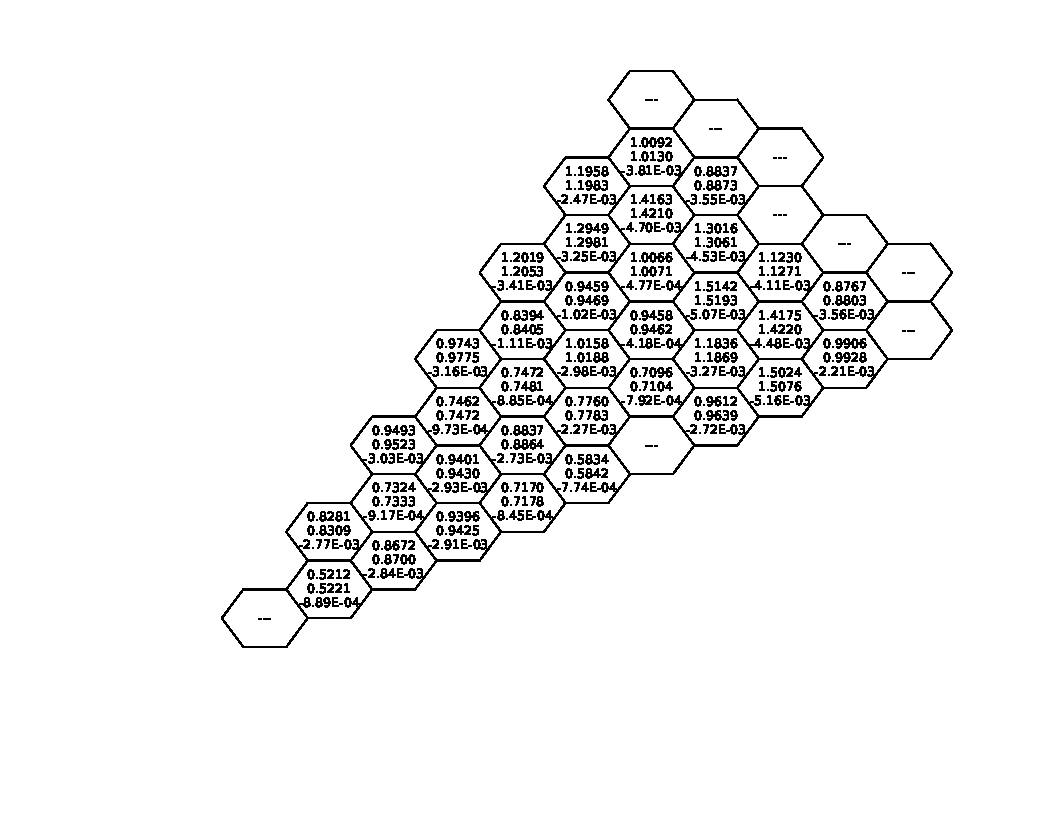
\includegraphics[width=\textwidth]{diffusion_vver440}
        \caption{VVER440 Benchmark Power Comparison for most refined mesh.}
        \label{fig:diffusion_vver440}
      \end{figure}
      \begin{table}
        \caption{VVER440 Benchmark Convergence Study. 
          $k_{ref} = 1.009700$ \cite{chao}}
        \label{tab:vver440}
        \begin{center}
          \begin{tabular}{cccc}
            \toprule
            Refine & $\keff$ & $\keff$ error [pcm] & $\keff$ ratio \\
            \midrule
            \csvreader[
              %head to column names,
              late after line=\\,
              late after last line=\\\bottomrule,]
              {ch02_neutronDiffusion/data/vver440.csv}{}
              {\csvcoli & \csvcolvi & \csvcolvii & \csvcolviii}
          \end{tabular}
        \end{center}
      \end{table}
    \subsubsection{SNR}
      \begin{figure}
        \centering
        \includegraphics[width=\textwidth]{diffusion_snr}
        \caption{SNR Benchmark Power Comparison for most refined mesh.}
        \label{fig:diffusion_snr}
      \end{figure}
      \begin{table}
        \caption{SNR Benchmark Convergence Study. 
          $k_{ref} = 1.124000$ \cite{argonneBenchmark}}
        \label{tab:snr}
        \begin{center}
          \begin{tabular}{cccc}
            \toprule
            Refine & $\keff$ & $\keff$ error [pcm] & $\keff$ ratio \\
            \midrule
            \csvreader[
              %head to column names,
              late after line=\\,
              late after last line=\\\bottomrule,]
              {ch02_neutronDiffusion/data/snr.csv}{}
              {\csvcoli & \csvcolvi & \csvcolvii & \csvcolviii}
          \end{tabular}
        \end{center}
      \end{table}
    \subsubsection{HWR}
      \begin{table}
        \caption{HWR Benchmark Convergence Study. 
          $k_{ref} = 0.991965$ \cite{chao}}
        \label{tab:hwr}
        \begin{center}
          \begin{tabular}{cccc}
            \toprule
            Refine & $\keff$ & $\keff$ error [pcm] & $\keff$ ratio \\
            \midrule
            \csvreader[
              %head to column names,
              late after line=\\,
              late after last line=\\\bottomrule,]
              {ch02_neutronDiffusion/data/hwr.csv}{}
              {\csvcoli & \csvcolvi & \csvcolvii & \csvcolviii}
          \end{tabular}
        \end{center}
      \end{table}
    \subsubsection{IAEA}
      % nore0125
      \begin{table}
        \caption{IAEA Benchmark Convergence Study. No Reflector. $\albedo = 
          0.125$. $k_{ref} = 0.991378 $ \cite{chao}}
        \label{tab:iaea_nore0125}
        \begin{center}
          \begin{tabular}{cccc}
            \toprule
            Refine & $\keff$ & $\keff$ error [pcm] & $\keff$ ratio \\
            \midrule
            \csvreader[
              %head to column names,
              late after line=\\,
              late after last line=\\\bottomrule,]
              {ch02_neutronDiffusion/data/iaea_nore0125.csv}{}
              {\csvcoli & \csvcolvi & \csvcolvii & \csvcolviii}
          \end{tabular}
        \end{center}
      \end{table}
      % nore0500
      \begin{table}
        \caption{IAEA Benchmark Convergence Study. No Reflector. $\albedo = 
          0.500$. $k_{ref} = 0.978077$ \cite{chao}}
        \label{tab:iaea_nore0500}
        \begin{center}
          \begin{tabular}{cccc}
            \toprule
            Refine & $\keff$ & $\keff$ error [pcm] & $\keff$ ratio \\
            \midrule
            \csvreader[
              %head to column names,
              late after line=\\,
              late after last line=\\\bottomrule,]
              {ch02_neutronDiffusion/data/iaea_nore0500.csv}{}
              {\csvcoli & \csvcolvi & \csvcolvii & \csvcolviii}
          \end{tabular}
        \end{center}
      \end{table}
      % refl0125
      \begin{table}
        \caption{IAEA Benchmark Convergence Study. With Reflector. $\albedo = 
          0.125$. $k_{ref} = 1.006630 $ \cite{chao}}
        \label{tab:iaea_refl0125}
        \begin{center}
          \begin{tabular}{cccc}
            \toprule
            Refine & $\keff$ & $\keff$ error [pcm] & $\keff$ ratio \\
            \midrule
            \csvreader[
              %head to column names,
              late after line=\\,
              late after last line=\\\bottomrule,]
              {ch02_neutronDiffusion/data/iaea_refl0125.csv}{}
              {\csvcoli & \csvcolvi & \csvcolvii & \csvcolviii}
          \end{tabular}
        \end{center}
      \end{table}
      % refl0500
      \begin{table}
        \caption{IAEA Benchmark Convergence Study. With Reflector. $\albedo = 
          0.500$. $k_{ref} = 1.005507 $ \cite{chao}}
        \label{tab:iaea_refl0500}
        \begin{center}
          \begin{tabular}{cccc}
            \toprule
            Refine & $\keff$ & $\keff$ error [pcm] & $\keff$ ratio \\
            \midrule
            \csvreader[
              %head to column names,
              late after line=\\,
              late after last line=\\\bottomrule,]
              {ch02_neutronDiffusion/data/iaea_refl0500.csv}{}
              {\csvcoli & \csvcolvi & \csvcolvii & \csvcolviii}
          \end{tabular}
        \end{center}
      \end{table}
  \subsection{Wedge Element Manufactured Solution Finite Cylinder}
      \begin{table}
        \caption{Three Dimension, One-Group, Criticality Convergence Study
          Results.}
        \label{tab:finite_cyl}
        \begin{center}
          \begin{tabular}{cccccccccc}
            \toprule
            Refine & $\keff$ & $\keff$ error [pcm] & $\keff$ ratio & RMS & 
              RMS ratio  & $\|e\|_{\infty}$ & $\|e\|_{\infty}$ ratio \\
            \midrule
            \csvreader[
              %head to column names,
              late after line=\\,
              late after last line=\\\bottomrule,]
              {ch02_neutronDiffusion/data/finite_cyl.csv}{}
              {\csvcoli & \csvcolii & \csvcoliii & \csvcoliv & \csvcolv & 
              \csvcolvi & \csvcolxi & \csvcolxii}
          \end{tabular}
        \end{center}
      \end{table}
  \subsection{Three Dimension Reactors}
    \subsubsection{MONJU}
      \begin{table}
        \caption{MONJU Benchmark Rod Worth Results.}
        \label{tab:monju}
        \begin{center}
          \begin{tabular}{cccccc}
            \toprule
            Pattern & $\keff$ & Rod Worth [pcm] & Rod Difference [\%$\Delta k$]&
              Rod Worth Error (relative) & Rod Difference Error [\%$\Delta k$]\\
            \midrule
            \csvreader[
              %head to column names,
              late after line=\\,
              late after last line=\\\bottomrule,]
              {ch02_neutronDiffusion/data/monju.csv}{}
              {\csvcoli & \csvcolii & \csvcoliii & \csvcoliv & \csvcolvi & 
              \csvcolvii}
          \end{tabular}
        \end{center}
      \end{table}
    \subsubsection{KNK}

\chapter{Neutron Diffusion Results}
\label{ch:diffusionResults}

\section{Introduction}
  This application of the FEM has been compared against reference 
  benchmark problems as well as analytic solutions. Comparison
  against benchmark problems demonstrates an ability to solve problems for
  which this application was intended. Comparison against analytic solutions 
  allows for more detailed error and convergence analysis as not only the system
  $\keff$ but also the flux solution are known exactly. 

  Running these comparisons serves as a verification and validation of this
  implementation of the FEM. The strategy used comes from \cite{oberkampf}. The
  first step is ``solution verification.'' Solution verification compares
  computational results to exact analytic results. Verification serves to
  demonstrate that the code itself is solving the correct equations as designed.
  This will be demonstrated with convergence to the analytic answer at the
  expected rate. The second step is ``solution validation.'' Solution validation
  compares computational results to benchmark results which may have been
  calculated computationally via another method or may come from experimental
  data. Validation demonstrates an ability to solve problems for which the
  method was originally intended. The data of the benchmark is not exact, but
  typically the solution has been verified by others previously.

  \begin{figure}
    \centering
    \includegraphics[width=\textwidth]{snr_paraview}
    \caption{Typical Two-Dimension Flux Visualization.}
    \label{fig:snr_paraview}
  \end{figure}

  \begin{figure}
    \centering
    \includegraphics[width=\textwidth]{monju3da_paraview}
    \caption{Typical Three-Dimension Flux Visualization.}
    \label{fig:monju3da_paraview}
  \end{figure}

\section{Error Analysis}
  For all reference problems presented, a convergence study is presented. It has 
  been shown that given a bounded second spatial derivative within the problem 
  domain, the FEM derived above is second-order convergent in space
  \cite{textbookli} (Remark 7.13). Mathematically, this is expressed
  \begin{equation} 
    \label{eq:error_bound}
    \|\ve\|_{\infty} \le c h^2 \| \grad^2 \phi(\vr) \|_{\infty}
  \end{equation}
  where $\ve$ is the error vector such that $\ve = \phi(\vr) - \phi_{FEM}$ and
  $\phi_{FEM}$ is solution to the finite element system of equations. In
  \eref{eq:error_bound} $h$ is the characteristic mesh size, and $c$ is a 
  constant.  \eref{eq:error_bound} implies that if the characteristic mesh size
  is halved, the error is quartered. This relationship is useful as a proper 
  implementation of the FEM must converge to the correct answer and do so at the 
  correct rate.
  
  Mesh refinement studies are presented herein. For each refinement, $h$ is 
  halved by introducing new elements and placing new nodes at the midway point
  between existing nodes. Then, let $i$ be the refinement index and the
  refinement ratio for a second-order convergent method is 
  \begin{equation}
    r = 4 = \frac{x^{(i-1)}}{x^{(i)}}
  \end{equation}
  such that for some quantity $x$, the error should theoretically decrease by a
  factor of four for each refinement. As these are numerical solutions, the 
  ratio rarely equals exactly four. It is observed that a few refinements are 
  often necessary before the ratio approaches the expected value. This is 
  especially the case when the second derivative is not bounded in problems with 
  heterogeneous materials.
  
  For benchmark problems, only $\keff$ is analyzed and expected to converge
  at the appropriate rate because the neutron flux solution is not known 
  exactly. When assembly powers were available, these are also
  presented graphically. In the graphical power representation, the key is 
  presented in \fref{fig:hex_description}.

  \begin{figure}
    \centering
    \includegraphics[width=0.2\textwidth]{hex_description}
    \caption{Key for Hexagonal Power Plots.}
    \label{fig:hex_description}
  \end{figure}
  
  For analytic solutions, the error of the function $\phi$ itself can be 
  analyzed because the solution is known exactly. The derivations of the exact 
  solutions are presented in \apref{ap:analyticSolutions}. For all analytic 
  problems, the Root Mean Squared (RMS) error as in \eref{eq:rms} is calculated
  for the error vector $\ve$ and is presented. The ratio between refinements 
  should assume the expected rate. RMS error is defined as
  \begin{equation} \label{eq:rms}
    \text{RMS}(\ve) = \sqrt{\frac{1}{N} \sum_{i=1}^{N} e_i}.
  \end{equation}
  The maximal norm $\| \cdot \|_{\infty}$ is also presented and the ratio 
  between refinements should assume the expected rate. The maximal norm of the
  error is defined as
  \begin{equation} \label{eq:infnorm}
    \|\ve\|_{\infty} = \max_{i=1,2,\ldots,N} \lvert e_i \rvert.
  \end{equation}
  For analytic criticality  problems, $\keff$ is also presented and the ratio 
  between refinements should assume the expected rate. $\keff$ error is 
  calculated with \eref{eq:keff_err} in units of Percent Mille \units{pcm} from 
  \eref{eq:pcm}.
  \begin{align}
    \label{eq:keff_err}
    \keff \; \text{ error } &= \kref - \keff \\
    \label{eq:pcm}
    x \units{pcm} &= x \times 10^5
  \end{align}

\section{Reference Results}
  Comparison of numerical solutions to analytical and benchmark solutions
  follow. Each of these sets of results include a mesh refinement study to
  observe the proper convergence at the expected rate of four.

  \subsection{Analytic Solutions}
    As a demonstration of the proper implementation of and solution to the 
    neutron diffusion equation, analytic solutions are derived and then 
    numerically computed. These are one-dimensional, two-dimensional, and 
    three-dimensional problems. These problems exercise both triangle and wedge 
    elements. For one-dimension problems a two-dimensional rectangular domain is
    used and, the top and bottom edges $y=0$ and $y=L_x$ are treated as mirror 
    boundary conditions to reduce the dimension of the problem. To verify there
    was no error obscured by this process, the results were reproduced for a 
    rotated problem with the left and right edges ($x=0$ and $x=L_x$) set to
    mirror boundary conditions as well.

    \subsubsection{One-Dimension, One-Group, Fixed Source}
      \label{sec:1dfixedsrc}
      Arguably the simplest solution to the neutron diffusion equation, this 
      problem  solves a domain $x \in [0,1]$ for a fixed unit source throughout
      the  problem. The exact solution is derived in \sref{sec:deriv_1dfixedsrc}
      and is presented in \eref{eq:analytic_1dfixedsrc}. Results 
      from the convergence study are presented in \tref{tab:1dfixedsrc}.
      \begin{table}
        \caption{One-Dimension, One-Group, Fixed Source Convergence Study 
          Results.}
        \label{tab:1dfixedsrc}
        \begin{center}
          \begin{tabular}{ccccc}
            \toprule
            Refine & RMS & RMS ratio & $\|e\|_{\infty}$ & 
              $\|e\|_{\infty}$ ratio \\
            \midrule
            \csvreader[
              late after line=\\,
              late after last line=\\\bottomrule,]
              {ch02_neutronDiffusion/data/1dfixedsrc.csv}{}
              {\csvcoli & \csvcolii & \csvcoliii & \csvcolviii & \csvcolix}
          \end{tabular}
        \end{center}
      \end{table}

    \subsubsection{One-Dimension, One-Group, Criticality}
      \label{sec:1d1g}
      This problem tests the calculation of the source term and the general 
      power iteration implementation in the solution method. This problem solves
      a fissile material in the domain $x \in [0,100]$.
      The exact solution is derived in \sref{sec:deriv_1d1g} and
      presented in \eref{eq:analytic_1d1g}. Results from
      the convergence study are presented in \tref{tab:1d1g}. The exact value 
      for the effective multiplication factor is $\kref = 1.998028$.
      \begin{table}
        \caption{One-Dimension, One-Group, Criticality Convergence Study
          Results.}
        \label{tab:1d1g}
        \begin{center}
          \begin{tabular}{cccccccccc}
            \toprule
            Refine & $\keff$ & $\keff$ error \units{pcm} & $\keff$ ratio & RMS & 
              RMS ratio  & $\|e\|_{\infty}$ & $\|e\|_{\infty}$ ratio \\
            \midrule
            \csvreader[
              late after line=\\,
              late after last line=\\,]
              {ch02_neutronDiffusion/data/1d1g.csv}{}
              {\csvcoli & \csvcolii & \csvcoliii & \csvcoliv & \csvcolv & 
              \csvcolvi & \csvcolxi & \csvcolxii}
            Ref. & 1.998028 \\
            \bottomrule
          \end{tabular}
        \end{center}
      \end{table}

    \subsubsection{Two-Dimension, One-Group, Criticality}
      This problem tests the ability to solve truly two-dimensional problems.
      The exact solution is derived in \sref{sec:deriv_2d1g} and
      presented in \eref{eq:analytic_2d1g}. Results from
      the convergence study are presented in \tref{tab:2d1g}. The exact value 
      for the effective multiplication factor is $\kref = 1.996060$.
      \begin{table}
        \caption{Two-Dimension, One-Group, Criticality Convergence Study
          Results.}
        \label{tab:2d1g}
        \begin{center}
          \begin{tabular}{cccccccccc}
            \toprule
            Refine & $\keff$ & $\keff$ error \units{pcm} & $\keff$ ratio & RMS & 
              RMS ratio  & $\|e\|_{\infty}$ & $\|e\|_{\infty}$ ratio \\
            \midrule
            \csvreader[
              late after line=\\,
              late after last line=\\,]
              {ch02_neutronDiffusion/data/2d1g.csv}{}
              {\csvcoli & \csvcolii & \csvcoliii & \csvcoliv & \csvcolv & 
              \csvcolvi & \csvcolxi & \csvcolxii}
            Ref. & 1.996060  \\
            \bottomrule
          \end{tabular}
        \end{center}
      \end{table}

    \subsubsection{One-Dimension, Two-Group, Criticality }
      This problem tests the solution of multigroup problems. The results 
      presented are the convergence of $\keff$ and the convergence of the ratio
      of relative magnitude of thermal to fast flux $\phi_2/\phi_1$.
      The exact solutions are derived in \sref{sec:deriv_1d2g} and
      the solutions are presented in \eref{eq:1d2g_1} and
      \eref{eq:1d2g_2}. Results from the convergence study are presented in 
      \tref{tab:1d2g}. The exact value for the effective multiplication factor 
      is $\kref = 0.892349$ and the exact value for the relative flux ratio
      is $(\phi_2/\phi_1)_{ref} = 0.261324$.
      \begin{table}
        \caption{One-Dimension, Two-Group, Criticality Convergence Study
          Results.}
        \label{tab:1d2g}
        \begin{center}
          \begin{tabular}{ccccccc}
            \toprule
            Refine & $\keff$ & $\keff$ error \units{pcm} & $\keff$ ratio & 
              $\phi_2/\phi_1$ & $\phi_2/\phi_1$ error & $\phi_2/\phi_1$ ratio \\
            \midrule
            \csvreader[
              late after line=\\,
              late after last line=\\,]
              {ch02_neutronDiffusion/data/1d2g.csv}{}
              {\csvcoli & \csvcolii & \csvcoliii & \csvcoliv & \csvcolv & 
              \csvcolvi & \csvcolvii}
            Ref. & 0.892349 &  &  & 0.261324 \\
            \bottomrule
          \end{tabular}
        \end{center}
      \end{table}

    \subsubsection{One-Dimension, One-Group, Two-Region, Criticality}
      This problem tests the mapping of materials to regions within the problem.
      The exact solution is derived in \sref{sec:deriv_2reg} and
      presented in \eref{eq:analytic_2reg}. Results from
      the convergence study are presented in \tref{tab:2reg}. The exact value 
      for the effective multiplication factor is $\kref = 0.962188$.
      \begin{table}
        \caption{One-Dimension, One-Group, Two-Region, Criticality Convergence
          Study Results.}
        \label{tab:2reg}
        \begin{center}
          \begin{tabular}{cccccccccc}
            \toprule
            Refine & $\keff$ & $\keff$ error \units{pcm} & $\keff$ ratio & RMS & 
              RMS ratio  & $\|e\|_{\infty}$ & $\|e\|_{\infty}$ ratio \\
            \midrule
            \csvreader[
              late after line=\\,
              late after last line=\\,]
              {ch02_neutronDiffusion/data/2reg.csv}{}
              {\csvcoli & \csvcolii & \csvcoliii & \csvcoliv & \csvcolv & 
              \csvcolvi & \csvcolxi & \csvcolxii}
            Ref. & 0.962188 \\
            \bottomrule
          \end{tabular}
        \end{center}
      \end{table}

    \subsubsection{Three-Dimension, One-Group, Finite Cylinder}
        This problem is a finite cylinder with zero-flux
        boundary conditions. The cylinder is three-dimensional but the solution
        can be reduced to two dimensions (radial and axial directions). 
        The exact solution is derived in \sref{sec:deriv_finite_cyl} and the
        solution is presented in \eref{eq:analytic_finite_cyl}. Results from the
        convergence study are presented in \tref{tab:finite_cyl}. The exact value
        for the effective multiplication factor is $\kref = 0.996711$.
        \begin{table}
          \caption{Finite Cylinder Convergence Study Results.}
          \label{tab:finite_cyl}
          \begin{center}
            \begin{tabular}{cccccccccc}
              \toprule
              Refine & $\keff$ & $\keff$ error \units{pcm} & $\keff$ ratio & RMS & 
                RMS ratio  & $\|e\|_{\infty}$ & $\|e\|_{\infty}$ ratio \\
              \midrule
              \csvreader[
                late after line=\\,
                late after last line=\\,]
                {ch02_neutronDiffusion/data/finite_cyl.csv}{}
                {\csvcoli & \csvcolii & \csvcoliii & \csvcoliv & \csvcolv & 
                \csvcolvi & \csvcolxi & \csvcolxii}
              Ref. & 0.996711 \\
              \bottomrule
            \end{tabular}
          \end{center}
        \end{table}

  \subsection{Benchmark Solutions}
    \label{sec:benchmark_solutions}
    The application presented here was designed simulate nuclear power reactors,
    both SFRs and other reactor designs. Two-dimension and three-dimension
    benchmark problems with similar reactor physics phenomena have been examined
    here. These problems come from existing benchmarks based on hexagonal 
    geometry. This collection of benchmarks represent various energy group 
    structures, geometries, assembly sizes,  boundary conditions, as well as 
    other properties. Data used in these problems is concisely presented in 
    \apref{ap:benchmarks}.
    
    For two-dimensional benchmarks, mesh refinement studies are provided and 
    convergence is observed relative to the reference $\keff$ value similar to
    analytic problems. For three-dimensional benchmarks, control rod worth
    measurement is instead used to observe agreement of the diffusion solution 
    to the benchmark solution. To measure control rod worth, three cases are run
    $\{A,B,C\}$ with control rods fully removed in case $A$, partially inserted
    in case $B$, and fully inserted in case $C$. Rod worth is presented in 
    units \units{$\Delta k$} and calculated as 
    \begin{equation}
      \label{eq:rodworth}
      \text{Rod Worth}_x = \frac{\keffsub{A} - \keffsub{x}}
        {\keffsub{A} \, \keffsub{x}}
    \end{equation}
    for $x = \{B,C\}$. That is, rod worth is always compared to the case with
    control rods fully removed, case $A$. Additionally, Rod Difference is
    presented in units \units{$\% \Delta$k} as
    \begin{align}
      \label{eq:roddifference}
      \text{Rod Difference} &= \keffsub{A} - \keffsub{x} \\
      x \% \Delta \text{k}  &= x \times 10^2
    \end{align}
    for $x = \{B,C\}$.


    \subsubsection{VVER440}
      Proposed in \cite{chao} and described in \sref{sec:vver440}, this
      benchmark, two-dimensional problem is based on a
      VVER-440 reactor. The VVER-440 is a 
      light-water moderated reactor and operates principally with thermal 
      neutron spectrum. Cross sections are provided for a two-group energy 
      structure.
      
      Power comparison between the most refined mesh and the reference solution 
      are presented graphically in \fref{fig:diffusion_vver440} according to the
      key in \fref{fig:hex_description}. Numerical mesh convergence study for 
      the quantity $\keff$ is presented in \tref{tab:vver440}.

      \begin{figure}
        \centering
        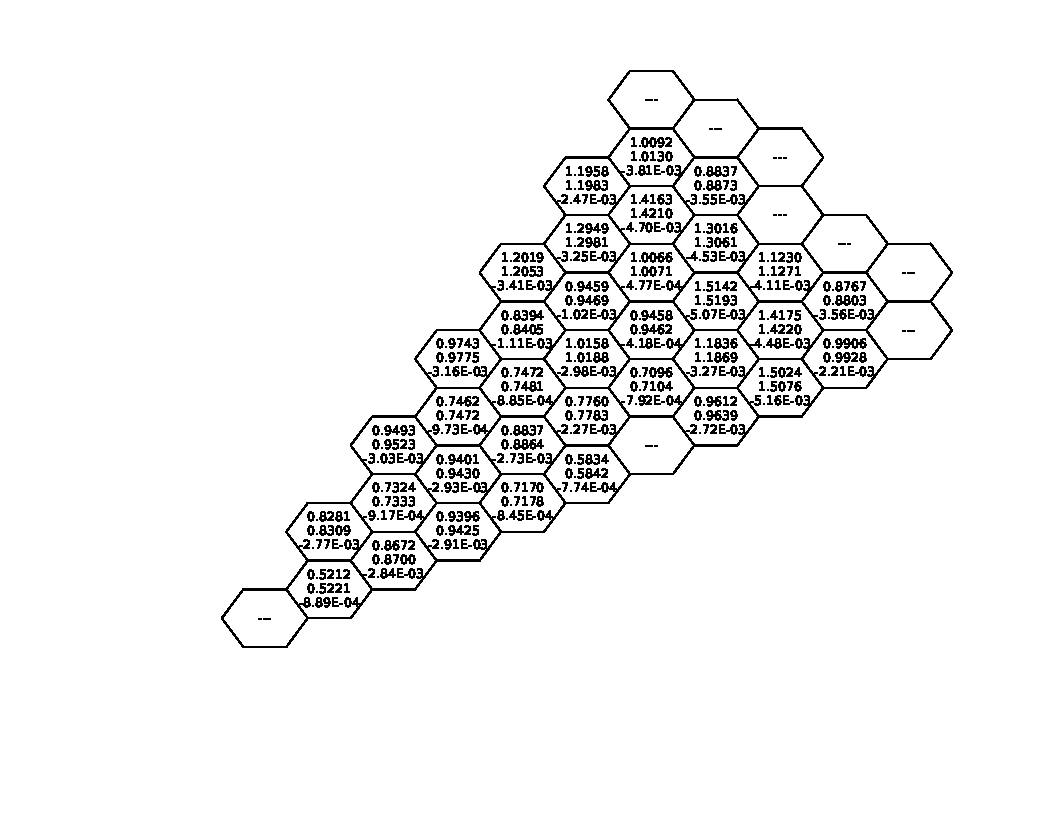
\includegraphics[width=\textwidth]{diffusion_vver440}
        \caption{VVER440 Benchmark Power Comparison for Most Refined Mesh.}
        \label{fig:diffusion_vver440}
      \end{figure}
      \begin{table}
        \begin{center}
          \caption{VVER440 Benchmark Convergence Study.}
          \label{tab:vver440}
          \begin{threeparttable}
            \begin{tabular}{cccc}
              \toprule
              Refine & $\keff$ & $\keff$ error \units{pcm} & $\keff$ ratio \\
              \midrule
              \csvreader[
                late after line=\\,
                late after last line=\\,]
                {ch02_neutronDiffusion/data/vver440.csv}{}
                {\csvcoli & \csvcolvi & \csvcolvii & \csvcolviii}
              Ref.\tnote{$\dagger$}  & 1.009700 \\
              \bottomrule
            \end{tabular}
            \begin{tablenotes}
              \item[$\dagger$] See \cite{chao}.
            \end{tablenotes}
          \end{threeparttable}
        \end{center}
      \end{table}

    \subsubsection{SNR}
      Proposed in \cite{argonneBenchmark} and described in \sref{sec:snr}, this
      benchmark, two-dimensional problem is based on a SNR reactor. The SNR
      is a sodium cooled fast reactor and operates principly with thermal
      neutrons. Cross sections are provided for a four-group energy structure.

      Power comparision between the most refined mesh and numerical solution
      given by DIF3D are presented graphicall in \fref{fig:diffusion_snr}
      according to the key in \fref{fig:hex_description}. Numerical mesh
      convergence study for the quantity $\keff$ is presented in \tref{tab:snr}.
      \begin{figure}
        \centering
        \includegraphics[width=\textwidth]{diffusion_snr}
        \caption{SNR Benchmark Power Comparison for Most Refined Mesh.}
        \label{fig:diffusion_snr}
      \end{figure}
      \begin{table}
        \begin{center}
          \caption{SNR Benchmark Convergence Study.}
          \label{tab:snr}
          \begin{threeparttable}
            \begin{tabular}{cccc}
              \toprule
              Refine & $\keff$ & $\keff$ error \units{pcm} & $\keff$ ratio \\
              \midrule
              \csvreader[
                late after line=\\,
                late after last line=\\,]
                {ch02_neutronDiffusion/data/snr.csv}{}
                {\csvcoli & \csvcolvi & \csvcolvii & \csvcolviii}
              Ref. \tnote{$\dagger$} & 1.124000 \\
              \bottomrule
            \end{tabular}
            \begin{tablenotes}
              \item[$\dagger$] See \cite{argonneBenchmark}.
            \end{tablenotes}
          \end{threeparttable}
        \end{center}
      \end{table}

    \subsubsection{HWR}
      Proposed in \cite{chao} and described in \sref{sec:hwr}, this
      benchmark, two-dimensional problem is based on a large Heavy Water
      Reactor (HWR). This is a heavy water moderated reactor and operates
      principally with thermal neutrons. Cross sections are provided for a
      two-group energy structure.

      Power comparison between the most refined mesh and the reference solution 
      are presented graphically in \fref{fig:diffusion_hwr} according to the
      key in \fref{fig:hex_description}. Numerical mesh convergence study for 
      the quantity $\keff$ is presented in \tref{tab:hwr}.
      \begin{figure}
        \centering
        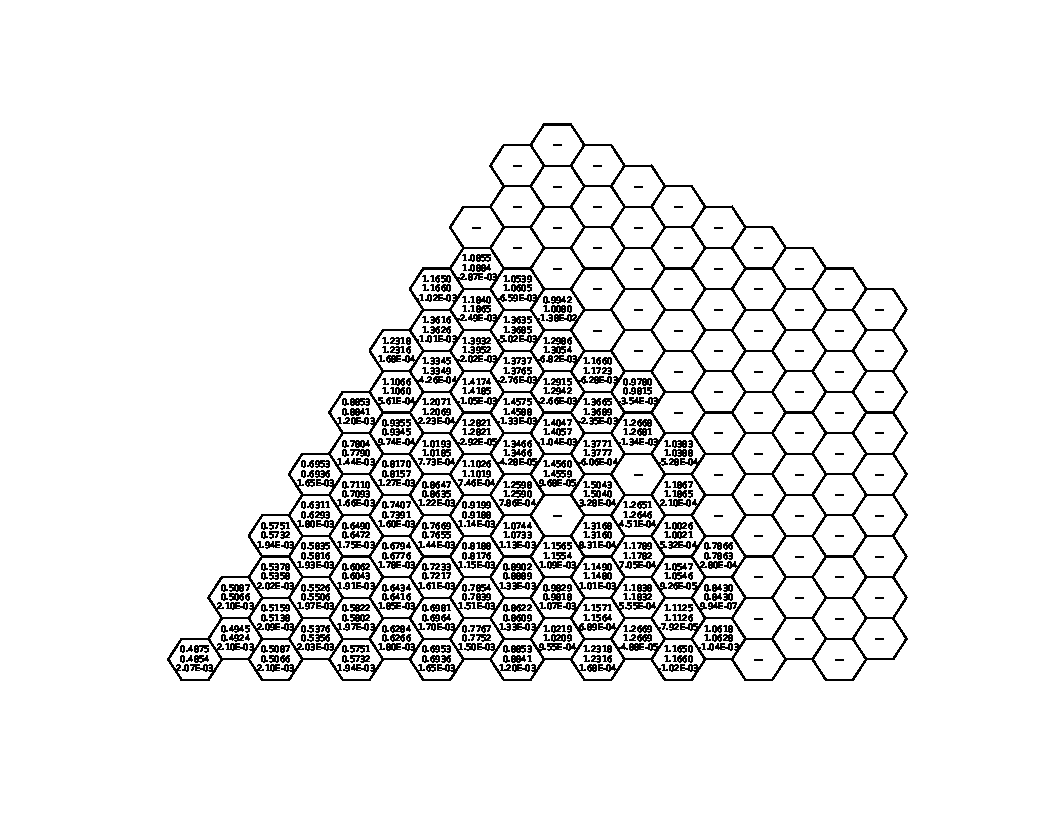
\includegraphics[width=\textwidth]{diffusion_hwr}
        \caption{HWR Benchmark Power Comparison for Most Refined Mesh.}
        \label{fig:diffusion_hwr}
      \end{figure}
      \begin{table}
        \begin{center}
          \caption{HWR Benchmark Convergence Study.}
          \label{tab:hwr}
          \begin{threeparttable}
            \begin{tabular}{cccc}
              \toprule
              Refine & $\keff$ & $\keff$ error \units{pcm} & $\keff$ ratio \\
              \midrule
              \csvreader[
                late after line=\\,
                late after last line=\\,]
                {ch02_neutronDiffusion/data/hwr.csv}{}
                {\csvcoli & \csvcolvi & \csvcolvii & \csvcolviii}
              Ref.\tnote{$\dagger$} & 0.991965  \\
              \bottomrule
            \end{tabular}
            \begin{tablenotes}
              \item[$\dagger$] See \cite{chao}.
            \end{tablenotes}
          \end{threeparttable}
        \end{center}
      \end{table}
    \subsubsection{IAEA}
      Proposed in \cite{chao} and described in \sref{sec:iaea}, this
      reactory-type, two-dimensional problem was originally based on a cartesian
      grid two-dimensional Pressurized Water Reactor (PWR) but was converted to
      hexagonal geometry in \cite{chao}. As it is based on a PWR deisgn, the
      reactor operates principally with thermal spectrum. Cross sections are
      provided for a two-group energy structure.

      The reactor is presented in four scenarios; both with and without
      reflective assemblies as well as with $\albedo = 0.125$ and $\albedo =
      0.5$. Numerical mesh convergence studies are presented for the quantity
      $\keff$ for each case in each of \tref{tab:iaea_nore0125},
      \tref{tab:iaea_nore0500}, \tref{tab:iaea_refl0125}, and
      \tref{tab:iaea_refl0500}.
      % nore0125
      \begin{table}
        \begin{center}
          \caption{IAEA Benchmark Convergence Study. No Reflector. $\albedo = 
            0.125$.}
          \label{tab:iaea_nore0125}
          \begin{threeparttable}
            \begin{tabular}{cccc}
              \toprule
              Refine & $\keff$ & $\keff$ error \units{pcm} & $\keff$ ratio \\
              \midrule
              \csvreader[
                late after line=\\,
                late after last line=\\,]
                {ch02_neutronDiffusion/data/iaea_nore0125.csv}{}
                {\csvcoli & \csvcolvi & \csvcolvii & \csvcolviii}
              Ref. \tnote{$\dagger$} & 0.991378 \\
              \bottomrule
            \end{tabular}
            \begin{tablenotes}
              \item[$\dagger$] See \cite{chao}.
            \end{tablenotes}
          \end{threeparttable}
        \end{center}
      \end{table}
      % nore0500
      \begin{table}
        \begin{center}
          \caption{IAEA Benchmark Convergence Study. No Reflector. $\albedo = 
            0.500$.}
          \label{tab:iaea_nore0500}
          \begin{threeparttable}
            \begin{tabular}{cccc}
              \toprule
              Refine & $\keff$ & $\keff$ error \units{pcm} & $\keff$ ratio \\
              \midrule
              \csvreader[
                late after line=\\,
                late after last line=\\,]
                {ch02_neutronDiffusion/data/iaea_nore0500.csv}{}
                {\csvcoli & \csvcolvi & \csvcolvii & \csvcolviii}
              Ref. \tnote{$\dagger$} & 0.978077 \\
              \bottomrule
            \end{tabular}
            \begin{tablenotes}
              \item[$\dagger$] See \cite{chao}.
            \end{tablenotes}
          \end{threeparttable}
        \end{center}
      \end{table}
      % refl0125
      \begin{table}
        \begin{center}
          \caption{IAEA Benchmark Convergence Study. With Reflector. $\albedo = 
            0.125$.}
          \label{tab:iaea_refl0125}
          \begin{threeparttable}
            \begin{tabular}{cccc}
              \toprule
              Refine & $\keff$ & $\keff$ error \units{pcm} & $\keff$ ratio \\
              \midrule
              \csvreader[
                late after line=\\,
                late after last line=\\,]
                {ch02_neutronDiffusion/data/iaea_refl0125.csv}{}
                {\csvcoli & \csvcolvi & \csvcolvii & \csvcolviii}
              Ref. \tnote{$\dagger$} & 1.006630 \\
              \bottomrule
            \end{tabular}
            \begin{tablenotes}
              \item[$\dagger$] See \cite{chao}.
            \end{tablenotes}
          \end{threeparttable}
        \end{center}
      \end{table}
      % refl0500
      \begin{table}
        \begin{center}
        \caption{IAEA Benchmark Convergence Study. With Reflector. $\albedo = 
          0.500$.}
        \label{tab:iaea_refl0500}
          \begin{threeparttable}
            \begin{tabular}{cccc}
              \toprule
              Refine & $\keff$ & $\keff$ error \units{pcm} & $\keff$ ratio \\
              \midrule
              \csvreader[
                late after line=\\,
                late after last line=\\,]
                {ch02_neutronDiffusion/data/iaea_refl0500.csv}{}
                {\csvcoli & \csvcolvi & \csvcolvii & \csvcolviii}
              Ref. \tnote{$\dagger$} & 1.005507 \\
              \bottomrule
            \end{tabular}
            \begin{tablenotes}
              \item[$\dagger$] See \cite{chao}.
            \end{tablenotes}
          \end{threeparttable}
        \end{center}
      \end{table}

    \subsubsection{MONJU}
      Proposed in \cite{monjuBenchmark} and described in \sref{sec:monju}, this 
      three-dimension, reactory-type problem is based on a Sodium-cooled Fast
      Reactor (SFR) operating principally with fast neutrons. Cross sections are
      provided for a three-group energy structure. However, the fission spectrum
      is not provided and is selcted for benchmark agreement. This assumed
      fission spectrum is presented in \tref{tab:monjuchi}. The rod worth
      measurements appear insensitive to fission spectrum. 

      Reference data can be found in \tref{tab:monjukeff}. Results from the
      finite element application are presented in \tref{tab:monju}. The error
      (difference between reference and calculated results) are presented in
      parenthesis next to the quantities. 
      Rod Worth is presented as calculated in \eref{eq:rodworth}. Rod Difference
      is presented as calculated in \eref{eq:roddifference}.

      \begin{table}
        \begin{center}
          \caption{MONJU Benchmark Rod Worth Results. \cite{monjuBenchmark}}
          \label{tab:monju}
          \begin{threeparttable}
            \begin{tabular}{ccll}
              \toprule
              Pattern & $\keff$ & Rod Worth \units{$\Delta k$} & 
                Rod Difference \units{\%$\Delta k$} \\
              \midrule
              A&1.056816&               &            \\
              B&1.031623&0.023 (2.51E-5) \tnote{$\dagger$} &2.52 (-0.07)\\
              C&1.006519&0.047 (1.77E-3)&5.03 (0.04) \\
              \bottomrule
            \end{tabular}
            \begin{tablenotes}
              \item[$\dagger$] Value in parentheses is difference to reference
                value from \cite{monjuBenchmark} as presented in 
                \sref{sec:monju}.
            \end{tablenotes}
          \end{threeparttable}
        \end{center}
      \end{table}
    \subsubsection{KNK}
      Proposed in \cite{takedaBenchmark} and described in \sref{sec:knk}, this
      three-dimension, benchmark problem is based on a SFR and is a model of
      the KNK-II core. Cross sections are provided for a four-group energy
      structure. There are many materials specified in the problem so it also
      aids in testing material mapping in a code. However, the reference data is
      for a transport solution. In this application, the transport cross
      sections are used to solve the neutron diffusion equation. This explains
      some of the numerical differences in the results but general trends are
      reflected. In addition to the comparison to the reference transport
      solution, the neutron diffusion equation is solved with DIF3D and the
      finite element results are comporable to the finite difference solution. 

      Reference data can be found in \tref{tab:knkkeff}. Results from the Finite
      Element neutron diffusion application are presented in \tref{tab:knk}. The
      error (difference between reference and calculated results) are presented
      in parenthesis next to the quantities.
      Rod Worth is presented as calculated in \eref{eq:rodworth}. Rod Difference
      is presented as calculated in \eref{eq:roddifference}.
      \begin{table}
        \begin{center}
          \caption{KNK Benchmark Rod Worth Results.}
          \label{tab:knk}
          \begin{threeparttable}
            \begin{tabular}{ccll}
              \toprule
              Pattern & $\keff$ & Rod Worth \units{$\Delta k$} & 
                Rod Difference \units{\%$\Delta k$} \\
              \midrule
              A&1.061752&               &            \\
              B&0.942404&0.119 (1.55E-2) \tnote{$\dagger$} &11.93 (0.75)\\
              C&0.829829&0.263 (3.99E-2)&23.19 (1.67)\\
              \bottomrule
            \end{tabular}
            \begin{tablenotes}
              \item[$\dagger$] Value in parentheses is difference to reference
                value from \cite{takedaBenchmark} as presented in 
                \sref{sec:knk}.
            \end{tablenotes}
          \end{threeparttable}
        \end{center}
      \end{table}

\chapter{Thermal Hydraulics}
\label{ch:thermalHydraulics}

\section{Introduction}
  For reactor design purposes, designs are ultimately constrained by thermal
  properties. Additionally, neutronics properties in the form of cross sections
  and density changes are significantly affected by system temperatures.
  Therefore, to accurately simulate the neutron distribution within the reactor,
  it is necessary to also simulate temperatures within the reactor.

  In this simulation, two thermal hydraulic models are
  employed. The first is a one-dimensional fluid flow model to calculate coolant
  temperatures as the coolant flows through a channel. This model is valid for
  the assumption of no cross-flow between channels and perfect fluid mixing 
  within the flow channel. For use in simulating fast reactors with canned
  assemblies and assembly designs which encourage mixing, these assumptions are
  valid. The second model used is a radial
  pin-conduction model to calculate cladding, sodium bond, and fuel temperatures
  based on the heat conduction equation.

  Thermodynamic properties of reactor materials are required for these models.
  The sodium properties required are the most extensive with density, enthalpy, 
  thermal conductivity, dynamic viscosity, and heat capacity required. The 
  functional forms of these properties in this application are given in 
  \cite{sodiumProp}. Additionally, thermal conductivity values are required for 
  cladding and fuel material. Typical cladding for fast reactor designs is HT9
  stainless steel and a functional form of the conductivity is given in
  \cite{ht9Prop}. Fuel composition is assumed to be of the form U-XZr where
  X is the weight fraction of Zr in the fuel. A typical value for X is 10\%.
  Fuel thermal conductivity is given in \cite{fuelProp}. For the expression of
  fuel thermal conductivity given, the integral of thermal conductivity 
  is unbounded as $T \rightarrow 0$ so thermal conductivity is assumed
  constant below 300 K which is below the melting point of sodium so this
  assumption is valid for reactor applications.

\section{Geometric Description}
  For the purposes of the thermal hydraulics model, geometry is described in
  \fref{fig:radial_model}. This model represents a cylindrical fuel pellet,
  surrounded by sodium bond, enclosed in steel cladding, with sodium coolant
  flowing in the axial direction. The center of the fuel pin is located at
  $r=0$ where $r$ is the radial coordinate. The fuel pellet has radius $R_F$ and
  fuel is located in $r \in [0,R_F)$. Then, bond is located in $r \in (R_F,R_B)$
  and clad is located in $r \in (R_B,R_C]$. The fuel center-line temperature is
  $T_0$ and fuel surface temperature is $T_F$. Bond surface temperature is
  $T_B$ and clad surface temperature is $T_C$. $T_{\infty}$ represents the bulk
  coolant temperature. In this model, heat is generated exclusively in the fuel
  with volumetric heat generation rate $q'''$. 

  In a cross-sectional assembly view, dimensions are presented in
  \fref{fig:pin_model} and \fref{fig:hex_can}. In \fref{fig:hex_can}, $Th_{Box}$
  is the thickness of the assembly box, F2F is the flat-to-flat measurement of
  the outside of the hexagonal can, and Pitch is the distance between the
  center of two pins. In future notation, the quantity ``Pitch'' is also noted
  $S$. Using the geometry described in these figures, the material
  cross-sectional areas are calculated according to the given formulae where
  $N_{pin}$ is the number of pins in the assembly.
  \begin{align}
    A_{total} &= \frac{\sqrt{3}}{2} F2F^2 \\
    A_{can} &= A_{total} - 
      \frac{\sqrt{3}}{2} \left(  F2F - 2 \, Th_{Box} \right) \\
    A_{wrap} &= N_{pin} \frac{\pi}{4} D_{wrap}^2 \\
    A_{clad} &= N_{pin} \pi (R_C^2 - R_B^2) \\
    A_{bond} &= N_{pin} \pi (R_B^2 - R_F^2) \\
    A_{fuel} &= N_{pin} \pi R_F^2 \\
    A_{cool} &= A_{total} - A_{can} - A_{wrap} - A_{clad} - A_{bond} - A_{fuel}
  \end{align}
  Calculating the areas as above allows for calculation of cross-sectional area
  fractions. Assuming constant dimensions within an element in the axial
  direction, these area fractions are equivalent to volume fractions and are
  useful for neutron cross section calculations. Additionally, these formulae
  allow for thermal expansion calculations as the liquid sodium in the bond and
  the coolant are allowed to vary to allow for the expansion of other materials.

  \begin{figure}
    \centering
    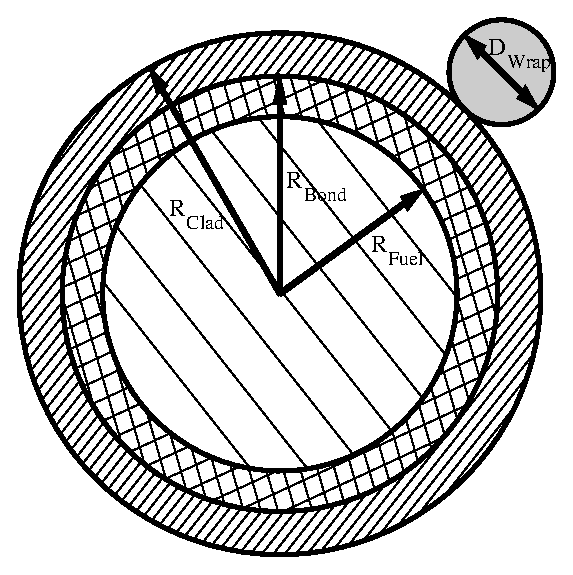
\includegraphics[width=0.5\textwidth]{pin_model}
    \caption{Dimensions of Thermal Hydraulic Pin Model.}
    \label{fig:pin_model}
  \end{figure}

  \begin{figure}
    \centering
    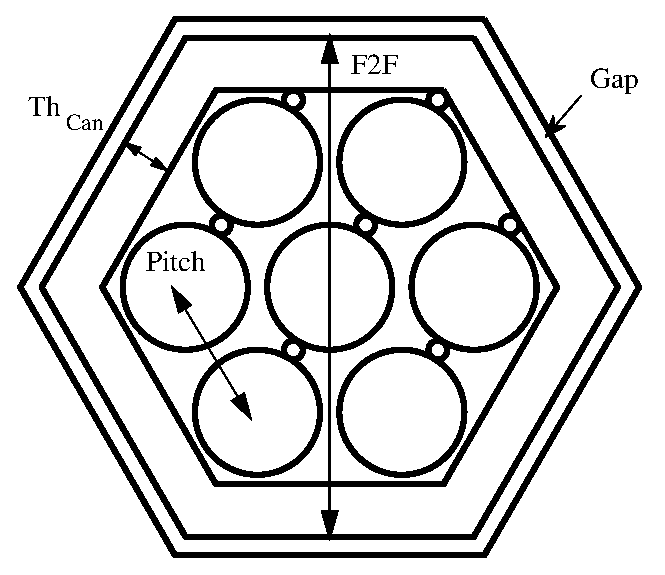
\includegraphics[width=0.5\textwidth]{hex_can}
    \caption{Dimensions of Hexagonal Can.}
    \label{fig:hex_can}
  \end{figure}
  
  \begin{figure}
    \centering
    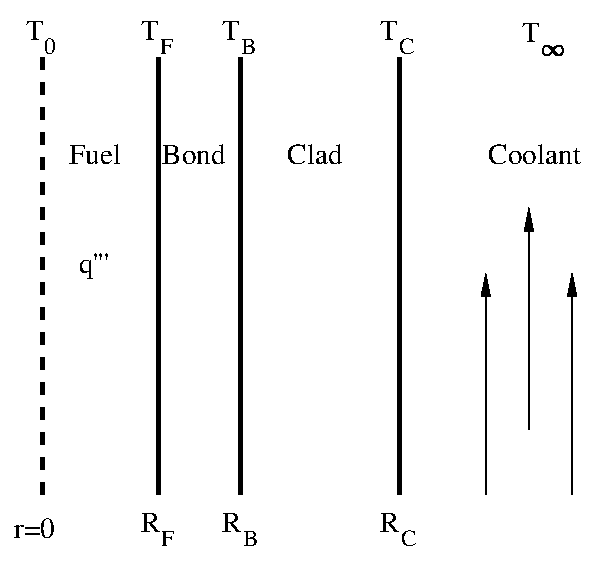
\includegraphics[width=0.5\textwidth]{radial_model}
    \caption{Geometry Description for Thermal Hydraulics Model.}
    \label{fig:radial_model}
  \end{figure}

  Used in association with an unstructured mesh, the thermal hydraulic model
  requires mapping mesh elements to flow channels. For the model described here,
  a flow channel is a single fuel assembly. In the user input to the
  program, the user must specify to which one-dimensional flow channel belongs.
  Adopting the nomenclature from fast reactors, each flow channel represents a
  hexagonal-assembly or a ``hex''. In the following discussion, a hex index is
  subscripted $h$ for $h = 1,2,\ldots,N_h$ where $N_h$ is the number of
  hexagonal assemblies in a reactor. Though the term ``hex'' is used, there is
  no assumption made in any of the calculations that the assembly is indeed
  hexagonal. Square one-dimensional assemblies would be simulated similarly.

  The concept of ``chunks'' is also introduced to aid in the discretization of
  the thermal hydraulic model. A chunk is the set of all elements in a channel
  with a unique axial elevation. For example, in a fast reactor hexagonal
  assembly, the assembly has a unique $h$ index and contains a number of chunks
  equal to the number of axial elevations in the simulation. Additionally, each 
  chunk is required to have unique material composition. The concept of chunks
  is shown in \fref{fig:chunk_description}.  Chunks are indexed
  $c = 1,2,\ldots,N_c$ where $N_c$ is the total number of chunks. For $N_z$
  axial elevations, $N_c = N_h \, N_z$. The indexing
  of chunks is chosen such that $c+N_h$ is the chunk one axial elevation above
  chunk $c$. 

  \begin{figure}
    \centering
    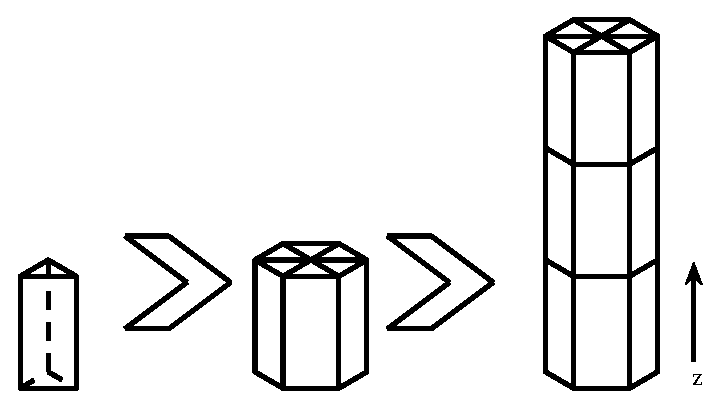
\includegraphics[width=0.7\textwidth]{chunk_description}
    \caption{Progression of Element (left), to Chunk (center), to Hex (right).}
    \label{fig:chunk_description}
  \end{figure}

\section{Power Calculation}
  Recall the multigroup neutron diffusion equation solved via the power
  iteration method returns the largest eigenvalue $\keff$ and unique positive
  eigenvector $\phi_g$ (see \sref{sec:power_iterations}). The flux calculated
  according to this method can be normalized to an arbitrary constant. For a
  specified total reactor power, $Q_{Rx}$ the normalization constant can be 
  calculated. For un-normalized neutron flux $\widetilde{\phi_{g,e}}$ with group
  $g$ in element $e$, the normalization constant is written as
  \begin{equation}
    \label{eq:normalization_c}
    c = \frac{Q_{Rx}}{\sum_{g}^{G} \sum_{e}^{N_E} \kappa \Sigma_{f,g,e} \,
      \widetilde{\phi_{g,e}}}
  \end{equation}
  where $c$ is the normalization constant. $\kappa$ represents the reclaimable
  (non-neutrino) energy produced per fission such that the quantity $\kappa
  \Sigma_f \phi$ represents the heat generation rate. Then the true reactor
  neutron flux is given as
  \begin{equation}
    \label{eq:normalization_phi}
    \phi_{g,e} = c \, \widetilde{\phi_{g,e}}
  \end{equation}
  and the power distribution is 
  \begin{equation}
    \label{eq:normalization_q}
    q_{e} = \sum_g^G \kappa \Sigma_{f,e,g} \phi_{g,e}.
  \end{equation}
  For an elemental power $q_e$, then the volumetric heat generation rate within
  the fuel is 
  \begin{equation}
    \label{eq:elementqppp_fuel}
    q'''_{e} = \frac{q_e}{V_{fuel,e}}
  \end{equation}
  where $V_{fuel,e}$ is the volume of fuel in element $e$. This will be
  necessary for the radial conduction model.

  For the one-dimensional heat convection model in the axial direction,
  heat generation quantities are needed for chunks instead of elements.
  The quantities required are then the total heat generated in a chunk $q_c$ and
  the average volumetric heat generation rate in the fuel for elements within
  the chunk $q'''_c$. These relationships are given in \eref{eq:chunkpwr} and
  \eref{eq:chunkqppp_fuel} respectively. The notation $e \in c$ implies the
  summation over all elements $e$ within chunk $c$.
  \begin{align}
    \label{eq:chunkpwr}
    q_c = \sum_{e \in c} q_e \\
    \label{eq:chunkqppp_fuel}
    q'''_c = \frac{\sum_{e \in c} q'''_e V_{fuel,e}}{\sum_{e \in c} V_{fuel,e}}
  \end{align}

\section{Axial Convection Model}
  \label{sec:axial_convection_model}
  First, the channel mass flow $\mdot_h$ must be calculated for a user specified
  total reactor mass flow rate $\mdot_{Rx}$.  Mass flow is partitioned into each
  channel assuming constant mass flux at the reactor inlet according to 
  \begin{equation}
    \label{eq:mass_flow_split}
    \mdot_h = \mdot_{Rx} \frac{A_{cool,h}}{A_{cool,Rx}}
  \end{equation}
  where $A_{cool,h}$ is the coolant flow area for channel $h$ and $A_{cool,Rx}$
  is the coolant flow area for the reactor.  That is, the mass 
  flow per unit area is assumed constant at the reactor inlet and the mass flow 
  in a channel is the product of the mass flux and the channel flow area. 
  
  The coolant enthalpy for an axial location $z$ within the channel is expressed
  by a simple heat balance equation as
  \begin{equation}
    \label{eq:continuous_heat_balance}
    h_h(x) = h_{in} + \frac{1}{\mdot_h} \int_0^z q'_h(z') \; dz'
  \end{equation}
  where $h$ is the specific enthalpy, $h_{in}$ is the inlet enthalpy, $\mdot_h$
  is the mass flow rate within the channel, and $q'_h(x)$ is the linear heat 
  generation rate for channel $h$ at elevation $z$. $h_{in}$ is related to a
  user specified 
  $T_{inlet}$ by a state relationship for the coolant $h_{in} = h(T_{inlet})$.
  The integral in \eref{eq:continuous_heat_balance} can be discretized along the
  channel and converted to a summation.
  \begin{equation}
    \label{eq:heat_balance}
    \widetilde{h_c} = 
      h_{in} + \frac{1}{\mdot_h} \sum_{i}^{N_z} q'_{i,h} \Delta z_{i,h}
  \end{equation}
  where $q'_{i,h}$ is the linear heat generation rate in the chunk located at 
  axial level $i$ in 
  channel $h$ and $\Delta z_{i,h} = z_{i+1,h} - z_{i,h}$. (Note: by indexing
  properly, $c = h + (i-1) \, N_h$.) Recognizing the 
  quantity $q'_{i,h} \Delta z_{i,h}$ is the total heat generated in channel $h$ 
  at axial level $h$, then \eref{eq:heat_balance} can be rewritten.
  \begin{equation}
    \widetilde{h_c} = h_{in} + \frac{1}{\mdot_h} \sum_i^{N_z} q_{i,h}
  \end{equation}
  The quantity $\widetilde{h_c}$ represents the enthalpy in channel $h$ at axial
  elevation $z_i$. Note that $z_i$ is the upper coordinate of the
  one-dimensional heat convection node. The node-average enthalpy is instead
  desired. To first-order approximation, then
  \begin{equation}
    h_c = \half (\widetilde{h_{i-1,h}} + \widetilde{h_{i,h}})
  \end{equation}
  where $h_c$ is the average enthalpy in chunk $c$ located in channel $h$ at
  axial level $i$.
  The final result of this model is $h_c$, the bulk coolant enthalpy in each
  chunk $c$. Given, $h_c$, bulk coolant temperature $T_{\infty,c} = T(h_c)$ can
  be calculated using a state relationship. This will be an input into the 
  Radial Conduction Model, \sref{sec:radial_conduction_model}, to later 
  calculate the average material temperatures.
  
\section{Radial Conduction Model}
  \label{sec:radial_conduction_model}
  \subsection{Surface Temperature and Center-Line Temperatures}
    \subsubsection{Fuel Center-Line Temperature}
      The fueled region is the only region modeled with non-zero volumetric heat
      generation. In this region, $q'''_c$ as specified by 
      \eref{eq:chunkqppp_fuel} is assumed constant within the fuel. 
      Additionally, the thermal conductivity in the fuel will be assumed to have
      general form $k_F(T)$. For this application, $k_F(T)$ is specified by the
      functional form in \cite{fuelProp} assuming 10\% Zr by weight included in
      fuel.

      The steady-state heat conduction equation with constant volumetric heat
      generation rate $q'''_c$ and variable thermal conductivity $k_F(T)$ can be
      written.
      \begin{equation}
        \label{eq:conduction_fuel}
        \grad \cdot (k_F(T) \grad T_F(r)) + q'''_c = 0
      \end{equation}
      Noting the gradient operator in cylindrical geometry,
      \eref{eq:conduction_fuel} is rewritten with partial derivatives.
      \begin{equation}
        \label{eq:conduction_fuel_cylindrical}
        \frac{1}{r} \frac{\partial}{\partial r} \left( r \, k_F(T) \, 
          \frac{d \, T_F}{dr} \right) + q'''_c = 0
      \end{equation}
      Note the inner derivative is an ordinary derivative because the only
      function to which it applies, $T_F(r)$, is a function of one variable. The
      outer derivative is a partial derivative because it applies to $T_F(r)$ as
      well as $k_F(T) = k_F(T_F(r))$.

      Begin solving \eref{eq:conduction_fuel_cylindrical} by multiplying the
      equation by radial coordinate $r$.
      \begin{equation}
        \frac{\partial}{\partial r} \left( k_F(T_F(r)) \, \frac{d\, T_F}{dr} 
        \right) + q'''_c = 0
      \end{equation}
      Integrate the equation for $r \in [0,r']$ where $r'$ is an arbitrary
      location $r' \in [0,R_F]$.
      \begin{align}
        \int_0^{r'} \left( \frac{\partial}{\partial r} \left( k_F(T_F(r)) \, 
          \frac{d\, T_F}{dr} \right) + q'''_c \right) \; dr &= 0 \\
        \int_0^{r'} \frac{\partial}{\partial r} \left( k_F(T_F(r)) 
          \frac{d \, T_F}{dr} \right) \; dr + \int_0^{r'} q'''_c \; dr &= 0 \\
        \left. r \, k_F(T_F(r)) \frac{d\,T_F}{dr} \right|_{r=0}^{r=r'} + 
          \left. \frac{q'''_c}{2} r^2 \right|_{r=0}^{r=r'} &= 0 \\
        \label{eq:dtdr_fuel}
        \left. r' k_F(T_F(r')) \frac{d\,T_F}{dr} \right|_{r=r'} + 
          \frac{q'''_c}{2} r^{\prime 2} &= 0
      \end{align}
      Divide by the location $r'$.
      \begin{equation}
        \left. k_F(T_F(r')) \frac{d \, T_F}{dr}\right|_{r=r'} + 
          \frac{q'''_c}{2} r' = 0
      \end{equation}
      Next, integrate $r' \in [0,r]$.
      \begin{align}
        \int_0^r \left( k_F(T_F(r')) \left. \frac{d\,T_F}{dr}\right|_{r=r'} 
          + \frac{q'''_c}{2} r' \right) \; dr' &= 0 \\
        \int_0^r k_F(T_F(r')) \left. \frac{d\,T_F}{dr}\right|_{r=r'} \; dr' + 
          \int_0^r \frac{q'''_c}{2} r' \; dr' &= 0 \\
        \int_0^r k_F(T_F(r')) \left. \frac{d\,T_F}{dr}\right|_{r=r'} \; dr' + 
          \left. \frac{q'''_c}{4} r^{\prime 2} \right|_{r'=0}^{r'=r} &= 0 \\
        \int_0^r k_F(T_F(r')) \left. \frac{d\,T_F}{dr}\right|_{r=r'} \; dr' + 
          \frac{q'''_c}{4} r^2 &= 0
      \end{align}
      The fundamental theorem of calculus allows for the expression of the first
      integral.
      \begin{equation}
        \label{eq:tcl_integral}
        \int_{T_F(0)}^{T_F(r)} k_F(T_F(r)) \; dr + \frac{q'''_c}{4} r^2 = 0
      \end{equation}
      In this derivation, $k_F(T)$ is allowed to be a generic function. 
      Therefore, \eref{eq:tcl_integral} does not have a simple forward 
      expression. Solving for $T_F(0)$ will require a non-linear search such as
      the bisection method. Define the conductivity integral of the generic
      conductivity function $k(T)$ as
      \begin{equation}
        \label{eq:conductivity_integral}
        K(T) = \int_0^T k(T') \; dT'.
      \end{equation}
      Then, \eref{eq:tcl_integral} can be rewritten.
      \begin{gather}
        K_F(T_F(r)) - K_F(T_F(0)) + \frac{q'''_c}{4} r^2 = 0 \\
        K_F(T_F(0)) = K_F(T_F(r)) + \frac{q'''_c}{4} r^2 \\
        \label{eq:tcl_conductivity_integral}
        K_F(T_F(0)) = K_F(T_F) + \frac{q'''_c}{4} R_F^2
      \end{gather}
      The fuel center-line temperature can be calculated using
      \eref{eq:tcl_conductivity_integral} given a functional form of the
      conductivity integral $K_F(T)$ by performing a search on the function
      where $T_F(0)$ is the fuel center-line temperature, $T_F=T_F(R_F)$ is the
      fuel surface temperature, and $R_F$ is the radius of the fuel. To
      calculate $T_F(0)$, the fuel surface temperature must be known.
      If more information is known about $K_F(T)$, a forward expression
      may be possible. However, a bisection method is implemented to maintain
      generality.

    \subsubsection{Fuel Surface Temperature}
      The fuel surface temperature is calculated by considering the heat
      conduction equation in the sodium bond region. There is no heat generation
      in this region so $q'''=0$.
      The steady-state heat conduction equation with no heat generation is
      written as
      \begin{equation}
        \label{eq:tc_grad}
        \grad \cdot (k_B(T_B(r)) \grad T_B(r)) = 0
      \end{equation}
      where $k_B(T)$ is a general expression for the thermal conductivity in the
      sodium bond and is given by a state relationship in \cite{sodiumProp}.
      $T_B(r)$ is the temperature within the cladding region.
      In this region, good thermal contact is
      assumed such that $T_F(R_F)=T_B(R_F)$. That is, the temperature is 
      continuous at the material discontinuity. Additionally, constant heat flux
      is assumed at the material discontinuity such that $k_F(T_F(R_F))
      \left.\frac{d\,T_F}{dr}\right|_{r=R_F} = k_B(T_B(R_F))
      \left.\frac{d\,T_B}{dr}\right|_{r=R_F}$.

      Recognizing cylindrical geometry, \eref{eq:tc_grad} can be rewritten.
      \begin{equation}
        \label{eq:tb_heat_conduction}
        \frac{1}{r} \frac{\partial}{\partial r} \left(
          r \, k_B(T_B(r)) \frac{d \, T_B}{dr} \right) = 0
      \end{equation}
      Begin solving \eref{eq:tb_heat_conduction} by multiplying the equation by
      the radial coordinate $r$.
      \begin{equation}
        \frac{\partial}{\partial r} \left( r \, k_B(T_B(r)) \frac{d \, T_B}{dr}
          \right) = 0
      \end{equation}
      Integrate the equation for $r \in[R_F,r']$ where $r'$ is an arbitrary
      location $r' \in [R_F,R_B]$.
      \begin{align}
        \int_{R_F}^{r'} \frac{\partial}{\partial r} \left( r\, k_B(T_B(r)) \, 
          \frac{d\,T_B}{dr} \right) \; dr &= 0\\
        \left. r\, k_B(T_B(r)) \frac{d\,T_B}{dr} \right|_{r=R_F}^{r=r'} &= 0 \\
        \label{eq:tf_first_integral}
        \left. r' \, k_B(T_B(r')) \frac{d\,T_B}{dr} \right|_{r=r'} - 
          \left. R_F \, k_B(T_B(R_F)) \frac{d\,T_B}{dr} \right|_{r=R_F} &= 0
      \end{align}
      The assumption of constant heat flux allows for the treatment of the
      spatial derivative at $R_F$. Recall from the derivation within the fuel
      region, the expression \eref{eq:dtdr_fuel} is exploited. The expression is
      valid for any $r' \in [0,R_F]$ so allow $r'=R_F$.
      \begin{align}
        \left. R_F k_F(T_F(R_F)) \frac{d\,T_F}{dr} \right|_{r=R_F} + 
          \frac{q'''_c}{2} R_F^2 &= 0 \\
        \label{eq:surface_relation}
        \left. R_F k_F(T_F(R_F)) \frac{d\,T_F}{dr} \right|_{r=R_F} &= 
          - \frac{q'''_c}{2} R_F^2
      \end{align}
      Recall from the earlier derivation that the quantity $q'''_c$ is the
      average volumetric heat generation rate within chunk $c$.
      \eref{eq:surface_relation} is substituted into
      \eref{eq:tf_first_integral}.
      \begin{equation}
        \label{eq:tf_first_bc}
        \left. r' \, k_B(T_B(r')) \frac{d\,T_B}{dr} \right|_{r=r'} +
          \frac{q'''_c}{2} R_F^2 = 0
      \end{equation}
      Divide \eref{eq:tf_first_integral} by the radial coordinate $r'$. This is
      valid because $r \ne 0$ in this region.
      \begin{equation}
        \left. k_B(T_B(r')) \frac{d\,T_B}{dr} \right|_{r=r'} + 
          \frac{q'''_c}{2} \frac{R_F^2}{r'} = 0
      \end{equation}
      Integrate the equation for $r' \in [R_F,r]$ where $r \in [R_F,r']$.
      \begin{align}
        \int_{R_F}^r \left( \left. k_B(T_B(r')) \frac{d\,T_B}{dr}\right|_{r=r'}
          + \frac{q'''_c}{2} \frac{R_F^2}{r'} \right) \; dr' &= 0 \\
        \int_{R_F}^r \left. k_B(T_B(r')) \frac{d\,T_B}{dr}\right|_{r=r'} \; dr'
          + \int_{R_F}^r \frac{q'''_c}{2} \frac{R_F^2}{r'} \; dr' &= 0\\
        \int_{R_F}^r \left. k_B(T_B(r')) \frac{d\,T_B}{dr}\right|_{r=r'} \; dr'
          + \frac{q'''_c}{2} R_F^2 \left. \ln(r') \right|_{r'=R_F}^{r'=r} &= 0\\
        \int_{R_F}^r \left. k_B(T_B(r')) \frac{d\,T_B}{dr}\right|_{r=r'} \; dr'
          + \frac{q'''_c}{2} R_F^2 ( \ln(r) - \ln(R_F)) &= 0 \\
        \int_{R_F}^r \left. k_B(T_B(r')) \frac{d\,T_B}{dr}\right|_{r=r'} \; dr'
          + \frac{q'''_c}{2} R_F^2 \ln\left(\frac{r}{R_F}\right) &= 0 
      \end{align}
      Again, the remaining integral can be rewritten by employing the
      fundamental theorem of calculus.
      \begin{equation}
        \label{eq:tf_fundamental_theorem}
        \int_{T_B(R_F)}^{T(r)} k_B(T_B(r)) \; dT + \frac{q'''_c}{2} R_F^2 
          \ln\left(\frac{r}{R_F}\right) = 0
      \end{equation}
      Defining a conductivity integral function $K_B(T)$ similar to
      \eref{eq:conductivity_integral}, \eref{eq:tf_fundamental_theorem} can be
      rewritten.
      \begin{gather}
        K_B(T_B(r)) - K_B(T_B(R_F)) + \frac{q'''_c}{2} R_F^2
          \ln\left(\frac{r}{R_F}\right) = 0 \\
        K_B(T_B(R_F)) = K_B(T_C(r)) + \frac{q'''_c}{2} R_F^2
          \ln\left(\frac{r}{R_F}\right) \\
        \label{eq:tf_conductivity_integral}
        K_B(T_F) = K_B(T_B) + \frac{q'''_c}{2} R_F^2
          \ln\left(\frac{R_B}{R_F}\right)
      \end{gather}
      The fuel surface temperature can be calculated using
      \eref{eq:tf_conductivity_integral} given a functional form of the
      conductivity integral $K_B(T)$ by performing a search on the function. In
      \eref{eq:tf_conductivity_integral}, $T_F=T_B(R_F)$ is the fuel surface 
      temperature, $T_B=T_B(R_B)$ is the bond surface temperature and must be
      given to use this expression.

    \subsubsection{Bond Surface Temperature}
      Consider the heat conduction equation in the cladding region. Derivation
      of the bond surface temperature $T_B=T_B(R_B)$ is similar to
      the fuel surface temperature because both consider a heat conduction
      equation with no heat generation. The steady-state heat conduction 
      equation for this region is written as
      \begin{equation}
        \label{eq:clad_conduction_grad}
        \grad \cdot (k_C(T_C(r)) \grad T_C(r)) = 0
      \end{equation}
      where $k_C(T)$ is a functional form of the thermal conductivity in the
      cladding from \cite{ht9Prop}. $T_C(r)$ is the temperature within the
      cladding region and $T_C=T_C(R_C)$ is the cladding surface temperature. 
      In this region, good thermal contact is assumed such that
      $T_B(R_B)=T_C(R_B)$. Additionally, constant heat flux is assumed at the
      cladding-bond boundary such that $\left. k_B(T_B(R_C))
      \frac{d\,T_B}{dr}\right|_{r=R_C} = \left. k_C(T_C(R_C))
      \frac{d\,T_C}{dr}\right|_{r=R_F}$.

      Rewriting the gradient for cylindrical geometry,
      \eref{eq:clad_conduction_grad}.
      \begin{equation}
        \label{eq:clad_conduction}
        \frac{1}{r} \frac{\partial}{\partial r} \left( r\, k_C(T_C(r)) 
          \frac{d\,T_C}{dr} \right) = 0
      \end{equation}
      Begin solving \eref{eq:clad_conduction} by multiplying the equation by the
      radial coordinate $r$.
      \begin{equation}
        \frac{\partial}{\partial r} \left( r\,k_C(T_C(r))\,\frac{d\,T_C}{dr}
          \right) = 0
      \end{equation}
      Integrate the equation through $r \in [R_B,r']$ where $r'$ is an arbitrary
      coordinate $r' \in [R_B,R_C]$.
      \begin{align}
        \int_{R_B}^{r'} \frac{\partial}{\partial r} \left( r \, k_C(T_C(r))
          \frac{d\,T_C}{dr} \right) \; dr &= 0 \\
        \left. r\,k_C(T_C(r)) \frac{d\,T_C}{dr} \right|_{r=R_B}^{r=r'} &= 0 \\
        \label{eq:clad_before}
        \left. r' \, k_C(T_C(r')) \frac{d\,T_C}{dr} \right|_{r=r'} - 
          \left. R_B \, k_C(T_C(R_B)) \frac{d\,T_C}{dr} \right|_{r=R_B} &= 0
      \end{align}
      The assumption of constant heat flux at the material discontinuity at
      $R_B$ allows for an expression of the derivative at $R_B$. Recall from the
      derivation within the bond region, the expression \eref{eq:tf_first_bc}
      can be used. The expression is valid for any $r' \in [R_F,R_B]$ so allow
      $r'=R_B$.
      \begin{align}
        \left. R_B \, k_B(T_B(R_B)) \frac{d\,T_B}{dr} \right|_{r=R_B} +
          \frac{q'''_c}{2} R_F^2 &= 0 \\
        \label{eq:clad_bc_relation}
        \left. R_B \, k_B(T_B(R_B)) \frac{d\,T_B}{dr} \right|_{r=R_B} &= 
          - \frac{q'''_c}{2} R_F^2
      \end{align}
      Recalling again that $q'''_c$ is the average volumetric heat generation
      rate in the fuel within chunk $c$. \eref{eq:clad_bc_relation} is
      inserted into \eref{eq:clad_before}.
      \begin{equation}
        \left. r' \, k_C(T_C(r')) \frac{d\,T_C}{dr} \right|_{r=r'} + 
          \frac{q'''_c}{2} R_F^2 = 0
      \end{equation}
      Divide by $r'$ because $r' \ne 0$ in this region.
      \begin{equation}
        \left. k_C(T_C(r')) \frac{d\,T_C}{dr} \right|_{r=r'} + 
          \frac{q'''_c}{2} \frac{R_F^2}{r'} = 0
      \end{equation}
      Integrate the equation for $r' \in [R_B,r]$ where $r \in [R_B,r']$.
      \begin{align}
        \int_{R_B}^r \left( \left. k_C(T_C(r')) \frac{d\,T_C}{dr} \right|_{r=r'}
          + \frac{q'''_c}{2} \frac{R_F^2}{r'} \right) \; dr' &= 0 \\
        \int_{R_B}^r \left. k_C(T_C(r')) \frac{d\,T_C}{dr} \right|_{r=r'} \; dr'
          + \int_{R_B}^r \frac{q'''_c}{2} \frac{R_F^2}{r'} \; dr' &= 0 \\
        \int_{R_B}^r \left. k_C(T_C(r')) \frac{d\,T_C}{dr} \right|_{r=r'} \; dr'
          + \frac{q'''_c}{2} R_F^2 \left. \ln(r') \right|_{r'=R_B}^{r'=r} &= 0\\
        \int_{R_B}^r \left. k_C(T_C(r')) \frac{d\,T_C}{dr} \right|_{r=r'} \; dr'
          + \frac{q'''_c}{2} R_F^2 (\ln(r) - \ln(R_B)) &= 0\\
        \int_{R_B}^r \left. k_C(T_C(r')) \frac{d\,T_C}{dr} \right|_{r=r'} \; dr'
          + \frac{q'''_c}{2} R_F^2 \ln\left(\frac{r}{R_B}\right) &= 0
      \end{align}
      Again, the integral term can be rewritten with use of the fundamental
      theorem of calculus.
      \begin{equation}
        \label{eq:clad_integral}
        \int_{T_C(R_B)}^{T_C(r)} k_C(T_C(r)) \; dr +
          \frac{q'''_c}{2} R_F^2 \ln\left(\frac{r}{R_B}\right) = 0
      \end{equation}
      Defining a conductivity integral function $K_C(T)$ similar to
      \eref{eq:conductivity_integral}, \eref{eq:clad_integral} can be rewritten.
      \begin{gather}
        K_C(T_C(r)) - K_C(T_C(R_B)) + \frac{q'''_C}{2} R_F^2
          \ln\left(\frac{r}{R_B}\right) = 0 \\
        K_C(T_C(R_B)) = K_C(T_C(r)) + \frac{q'''_c}{2} R_F^2
          \ln\left(\frac{r}{R_B}\right) \\
        \label{eq:ktb}
        K_C(T_B) = K_C(T_C) + \frac{q'''_C}{2} R_F^2
          \ln\left(\frac{R_C}{R_B}\right) 
      \end{gather}
      The bond surface temperature can be calculated using \eref{eq:ktb} given a
      function describing the cladding conductivity integral $K_C(T)$ and
      performing a bisection method search on the function. In \eref{eq:ktb},
      $T_B = T_C(R_B)$ is the bond surface temperature, $T_C=T_C(R_C)$ is the
      clad surface temperature and is calculated using a different method and
      treated as an input to this method.  

    \subsubsection{Clad Surface Temperature}
      Clad surface temperature $T_C$ is given by Newton's Law of Cooling with
      convective heat transfer coefficient $h_c$ specified according to the
      Weisman Correlation. Newton's Law of Cooling may be written as
      \begin{equation}
        q''_{clad} = h_c (T_C - T_{\infty})
      \end{equation}
      where $q''_{clad}$ is the heat flux at the clad surface $R_C$, $h_c$ is
      the convective heat transfer coefficient, $T_C$ is the clad surface
      temperature, and $T_{\infty}$ is the bulk coolant temperature. Using the
      relationships in \sref{sec:axial_convection_model}, $T_{\infty}$ is given
      by the state relationship $T_{\infty} = T(h_c)$. The heat flux at the clad
      surface is related to the volumetric heat generation rate in the fuel
      according to 
      \begin{equation}
        q''_{clad} = q'''_c \frac{R_F^2}{2 R_C}
      \end{equation}
      where $q'''_c$ is the chunk-average volumetric heat generation rate in the
      fuel according to \eref{eq:chunkqppp_fuel}.

      The coefficient $h_c$ must be calculated via an applicable correlation.
      The Weisman correlation is selected because it is valid for general fluid
      flow and has parameters correlated for triangular pitch flow areas common
      to fast reactor designs. The Weisman Correlation relates the Nusselt,
      Reynolds, and Prandlt dimensionless numbers according to
      \begin{equation}
        \label{eq:weisman}
        Nu = C \, Re^{0.8} \, Pr^{1/3}
      \end{equation}
      where $Nu$ is the Nusselt number, $Re$ is the Reynolds number, $Pr$ is 
      the Prandlt number, and $C$ is a correlation coefficient specified by the
      triangular geometry. For triangular pitch flow, the geometry is described
      as
      \begin{align}
        \label{eq:weisman_c}
        C &= 0.026 \frac{S}{2 \, R_C} - 0.006 \\
        \label{eq:weisman_ax}
        A_x &= \frac{\sqrt{3}}{4} S^2 - \frac{\pi R_C^2}{2} \\
        \label{eq:weisman_pw}
        P_w &= \pi R_C \\
        \label{eq:weisman_de}
        D_e &= \frac{4 \, A_x}{P_w}
      \end{align}
      where $S$ is the pitch between pins (see \fref{fig:hex_can}), $A_x$ is the
      flow cross-sectional area, $P_w$ is the flow wetted perimeter, and $D_e$
      is the effective flow diameter. The Reynolds number is defined as
      \begin{equation}
        \label{eq:re}
        Re = \frac{\mdot_h \, D_e}{A_x \, \mu}
      \end{equation}
      where $\mdot_h$ is the assembly mass flow rate, $\mu$ is the fluid's
      dynamic viscosity given by a state relationship, and $D_e$ and $A_x$ are 
      defined according to \eref{eq:weisman_de} and \eref{eq:weisman_ax}
      respectively. The Prandtl number is defined according to 
      \begin{equation}
        \label{eq:pr}
        Pr = \frac{c_p \, \mu}{k}
      \end{equation}
      where $c_p$ is the fluid specific heat capacity at constant pressure, 
      $\mu$ is the fluid dynamic viscosity, and $k$ is the fluid thermal 
      conductivity. Note that each of these quantities are given by state 
      relationships. As such, the Prandtl number can itself be correlated for a
      given fluid as a state relationship.
      
      With the dimensionless quantities expressed in \eref{eq:re} and
      \eref{eq:pr}, the Weisman correlation is used to calculate the Nusselt
      number. Given a Nusselt number, the convective heat transfer coefficient
      is defined as
      \begin{equation}
        \label{eq:hc}
        h_c = \frac{Nu \, k}{D_e}
      \end{equation}
      where $Nu$ is the Nusselt number from the Weisman correlation
      \eref{eq:weisman}, $k$ is the fluid thermal conductivity given by a state
      relationship, and $D_e$ is the effective flow diameter given in
      \eref{eq:weisman_de}. Finally, the clad surface temperature is expressed.
      \begin{align}
        T_C &= \frac{q''_{clad}}{h_c} + T_{\infty} \\
        \label{eq:tc}
        T_C &= q'''_c \frac{R_F^2}{2\,R_c\,h_c} + T_{infty}
      \end{align}

  \subsection{Average Temperatures}
\section{Cross Section Treatment}
  \subsection{Cross Section Library Generation}
  \subsection{Temperature Dependent Cross Section Calculation}

% todo this will probably be a separate chapter and include thermal expansion
%\section{Results}
%  \subsection{Single Pin Model}
%  \subsection{Reactor Simulation}

\chapter{Thermal Expansion}
\label{ch:thermalExpansion}

\section{Necessity of Modeling}
  The Fast Reactor (FR) as modeled is entirely composed of
  metals and, as such, experiences significant thermal expansion. While other 
  designs may employ non-metallic fuel material (e.g. oxides or carbides), these 
  are not considered. Reactor designs composed of metal fuel include 
  Experimental Breeder Reactor II (EBR-II) as designed and built by Argonne 
  National Laboratory (ANL) and PRISM as designed by GE-Hitachi Nuclear Energy 
  (GEH).

  In metal fueled reactors such as EBR-II and PRISM, thermal expansion 
  represents a significant reactivity effect and requires modeling. PRISM 
  estimates a thermal expansion feedback such that a 1\% change in radial 
  dimension results in $-0.5 \units{$\Delta k$}$ indicating a significant effect 
  \cite{GEFR793}. Additionally, thermal expansion has been proven to serve as an 
  inherent safety feature of SFRs. In the remarkable EBR-II demonstrations in 
  April 1986, two major accident events were performed on the reactor while 
  operating at full power. Operators forced the reactor to undergo Unprotected 
  Loss-Of-Flow (ULOF) and Unprotected Loss-Of-Heat-Sink (ULOHS) events. EBR-II 
  was safely shutdown due to nothing other than inherent thermal feedback 
  effects. These experiments demonstrated conclusively the passive safety of SFR
  designs due in part to the thermal expansion of materials 
  \cite{PlentifulEnergy}.

\section{Model Details}
  \label{sec:model_details}
  Highly detailed thermal expansion modeling can be performed using the Finite
  Element Method (FEM) to calculate local stresses and strains on all reactor
  structural components. However, the model developed here for the simulation of
  fast reactors does not estimate temperature and heat generation at all 
  positions due to the smearing of hexagonal assemblies. Therefore, a simplified 
  thermal expansion model is developed to simulate the effect of thermal 
  expansion on reactivity.

  In the model, linear dimensions are expanded based on material properties.
  All sodium in the reactor is assumed to be liquid so effects of thermal
  expansion within the sodium are assumed to be described by the change in
  density as a function of temperature as described by state equations in
  \cite{sodiumProp}. Additionally, the mass of sodium within the reactor is not
  conserved. In a Sodium-cooled Fast Reactor (SFR), sodium in the coolant is 
  allowed to flow into and out of an expansion vessel external to the reactor.
  The sodium in the bond region flows upward from the fuel region into a gas 
  plenum at the top of the fuel rod as the fuel expands. However, this is not 
  modeled as the sodium level in the bond is not tracked. Instead, the mass of 
  sodium in the bond region is allowed to vary during the simulation.

  \subsection{Material Properties}
    \label{sec:model_details__material_properties}
    All structural materials in the reactor are modeled as HT9 stainless steel.
    Fuel material is modeled as metallic uranium with 10\% Zr by weight included
    (i.e. U10Zr). Thermal expansion properties for HT9 are given in 
    \cite{ht9Prop} and for U10Zr are given in \cite{thexpU10Zr}. The equations 
    for the Linear Expansion Factor (LEF) as functions of temperature and used 
    in this implementation are given
    \begin{equation}
      \label{eq:lef_ht9}
      \left( \frac{\Delta L}{L} \right)_{\text{HT9}} = 
        -2.191 \times 10^{-3} + 5.678 \times 10^{-6} \, T + 
        8.111 \times 10^{-9} \, T^2 - 2.576 \times 10^{-12} \, T^3 ,
    \end{equation}
    \begin{multline}
      \label{eq:lef_u10zr}
      \left( \frac{\Delta L}{L} \right)_{\text{U10Zr}} = \\
        \begin{cases}
          -7.3 \times 10^{-3} + 3.489 \times 10^{-5} \, T 
            - 5.154 \times 10^{-8} \, T^2 + 4.39 \times 10^{-11} \, T^3 & 
            T \le 923 \units{K} \\
          -0.25252 + 6.669 \times 10^{-4} \, T - 5.441 \times 10^{-7} \, T^2 
            + 1.518 \times 10^{-10} \, T^3 & \text{otherwise}
        \end{cases}
    \end{multline}
    for $T$ in \units{K}. Note that U10Zr undergoes a phase change at 
    $923 \units{K}$ that increases the LEF at this point. The LEF of HT9 and 
    U10Zr over the range of operating temperatures of fast reactors are plotted 
    in \fref{fig:lef_plot}. It is observed that the LEF of U10Zr is as much as 
    twice that of HT9. This implies fuel material will expand significantly more 
    than structural material which is expected behavior for metallic fuel.

    \begin{figure}
      \centering
      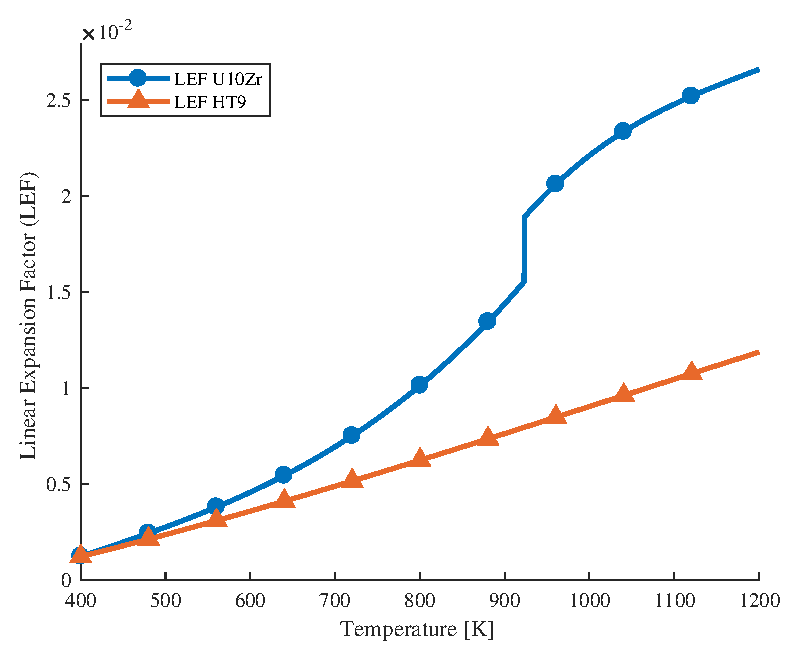
\includegraphics[width=0.7\textwidth]{lef_plot}
      \caption{Linear Expansion Factor for HT9 Steel and U10Zr Fuel.}
      \label{fig:lef_plot}
    \end{figure}
    
  \subsection{Assumptions and Formulae}
  \label{sec:model_details__assumptions_and_formulae}
    To simplify the modeling of thermal expansion, material dimensions are
    uniformly expanded in radial and axial directions. It is assumed that 
    material expansion in the radial direction (both $x$ and $y$ directions) 
    expands as HT9 because the dominating expansion in this direction is due to 
    the expansion of the hexagonal assemblies themselves and the grid plate at
    the base of the reactor. The exception to radial thermal expansion is that 
    the radius of the fuel, $R_F$, expands as U10Zr.  Within a hexagonal 
    assembly, the coolant flow area and the sodium bond area are allowed to 
    vary because they are assumed liquid.  It is assumed that material 
    expansion in the axial direction (the $z$ direction) expands as U10Zr 
    because the dominating expansion in this direction is the elongation of the 
    metallic fuel. 
    
    All dimensions in the reactor are expanded assuming the user-input 
    dimensions are at room-temperature conditions. Dimensions are expanded
    according to two user-input temperatures, $\texpfuel$ and $\texpstruct$.
    $\texpfuel$ corresponds to the average temperature of reactor fuel and
    $\texpstruct$ corresponds to the average temperature of steel in the
    reactor. Typically, these values come from a previous coupled diffusion and
    thermal hydraulics simulation.
    It is expected thermal expansion 
    effects will be significant. However, thermal expansion factors are 
    typically on the order $10^{-6}$ so small, local changes in temperature are 
    not expected to affect the macroscopic simulation.

    Given the assumptions of this model, a radial LEF can be defined using 
    \eref{eq:lef_ht9} as
    \begin{equation}
      \label{eq:lef_r}
      F_r(\texpstruct) = \left(\frac{\Delta L}{L}\right)_{\text{HT9}}
    \end{equation}
    which is a function of $\texpstruct$. Note that given the assumption of 
    uniform radial thermal expansion, ${F_x(\texpstruct) = F_y(\texpstruct) =
    F_r(\texpstruct)}$.
    Similarly, an axial LEF can be defined using \eref{eq:lef_u10zr} as 
    \begin{equation}
      \label{eq:lef_a}
      F_a(\texpfuel) = \left(\frac{\Delta L}{L}\right)_{\text{U10Zr}}
    \end{equation}
    and $F_a(\texpfuel) = F_z(\texpfuel)$. For a ``cold'' cooridnate 
    $(x^C,y^C,z^C)$, the thermally expanded ``hot'' coordinate $(x^H,y^H,z^H)$ 
    can be expressed using radial and axial LEFs as
    \begin{align}
      \label{eq:expand_x}
      x^H &= x^C + x^C \, F_r(\texpstruct) \\
      \label{eq:expand_y}
      y^H &= y^C + y^C \, F_r(\texpstruct) \\
      \label{eq:expand_z}
      z^H &= z^C + z^C \, F_a(\texpfuel)
    \end{align}
    which is consistent with the assumption of uniform radial and axial 
    expansion. These formulae expand the distance from each coordinate to the
    origin, $(0,0,0)$.

    Using the coordinate transforms in \eref{eq:expand_x}, \eref{eq:expand_y}, 
    and \eref{eq:expand_z}, consider the thermal expansion of a cold volume 
    $V^C$.  Volume $V^C$ has coordinate components $L_x^C$, $L_y^C$, and $L_z^C$
    such that ${V^C = L_x^C \, L_y^C \, L_z^C}$. Then, the thermally expanded 
    volume $V^H$ can be written
    \begin{align}
      V^H &= V^C + \Delta V, \\
      V^H &= (L_x^C + \Delta L_x) (L_y^C + \Delta L_y) (L_z^C + \Delta L_z). 
    \end{align}
    Then, recognizing the coordinate expansions,
    \begin{align}
      V^H &= (L_x^C + L_x^C \, F_r(\texpstruct)) + 
        (L_y^C + L_y^C \, F_r(\texpstruct)) + 
        (L_z^C + L_z^C \, F_a(\texpfuel)), \\
      V^H &= L_x^C \, L_y^C \, L_z^C \, (1 + F_r(\texpstruct))^2
        (1+F_a(\texpfuel)), \\
      V^H &= V^C (1 + F_r(\texpstruct))^2 (1+F_a(\texpfuel)).
    \end{align}
    The volume ratio is then
    \begin{equation}
      \label{eq:volume_ratio}
      \frac{V^C}{V^H} = \frac{1}{(1+F_r(\texpstruct))^2 (1+F_a(\texpfuel))}.
    \end{equation}
    Given the assumption of uniform thermal expansion in axial and radial
    directions, the ratio of volumetric expansion is constant throughout the
    reactor.

    The hexagonal assembly has total cross-sectional area $A$ and contains 
    component cross sections with areas $A_i$. For example, the total area 
    occupied by the fuel material could be considered $A_i$ and the total area 
    of the hexagon described by the flat-to-flat dimension could be considered 
    $A$. Define $A_i$ such that $\sum_{i} A_i = A$. Let the fractional area 
    $a_i = A_i/A$ and $\sum_{i} a_i = 1$.

    Using a method similar to the derivation of the volume ratio, a ratio can be
    derived for thermally expanded areas and area fractions. However, this would
    not be useful to the model because within an assembly, not all dimensions
    expand uniformly within the radial direction.
    The fuel radius and fuel area are expanded according to 
    $\left(\frac{\Delta L}{L_0}\right)_{\text{U10Zr}}$ whereas all other 
    materials are expanded according to 
    $\left(\frac{\Delta L}{L_0}\right)_{\text{HT9}}$. This does imply that,
    numerically, the radius of the fuel could exceed the inner radius of the 
    clad which is a non-physical result. This will only happen for small sodium 
    bond gaps and high thermal expansion temperatures. In these cases, the 
    radius of the fuel is confined to the expanded inner radius of the cladding.
    Though a more complex relationship describes the true value of these radii, 
    the error due to this assumption is small compared to the assumption of 
    uniform thermal expansion.
    
    Due to the different thermal expansions of fuel and structural material 
    within the cross-sectional area of the hexagonal assembly, the thermal 
    expansion of area fractions does not have a general formulaic relationship.
    Instead, area fractions are simply calculated at hot and cold conditions
    using expanded and unexpanded dimensions respectively. 

\section{Implementation}
  Thermal expansion affects the reactor in two major ways. First, thermal 
  expansion causes the physical dimensions of the reactor to increase. This is 
  modeled by the expansion of individual elements in the solution of the neutron 
  diffusion equation via the finite element method 
  (see \chref{ch:neutronDiffusion}) as well as the expansion of areas within the 
  hexagons. Second, as a result in the increase in physical dimensions, the 
  density of reactor materials decreases. This decrease in density is necessary
  to preserve the quantity of material within the reactor. In this derivation,
  the number of atoms in the reactor are conserved. The density change due to 
  thermal expansion is observed as a decrease in cross-sections.

  \subsection{Expansion of Elements and Area Fractions}
    Given the assumption of constant thermal expansion in radial and axial
    directions, thermal expansion follows immediately. Each node coordinate in
    the unstructured mesh is expanded according to \eref{eq:expand_x}, 
    \eref{eq:expand_y}, and \eref{eq:expand_z}. By expanding in axial and radial
    directions uniformly throughout the reactor, it is certain that there will 
    be no intersection or overlap of elements. In a realistic analysis, stress,
    strain, contact pressures, et cetera must be accounted for but this is 
    unnecessary here because the assumptions prohibit overlap and intersection 
    conditions.  As previously discussed in
    \sref{sec:model_details__assumptions_and_formulae}, the thermal expansion of
    area fractions is calculated directly.

  \subsection{Cross-section Effects}
    \label{sec:cross-section_effects}
    The conservation of reactor material is expressed as a conservation of 
    number of atoms. Allow the superscript $H$ to represent ``hot'' conditions 
    (i.e.  thermally expanded) and the superscript $C$ to represent ``cold'' 
    conditions.  Then, the conservation of the number of atoms for species $i$, 
    can be expressed as
    \begin{equation}
      \label{eq:conservation}
      n_i^H = n_i^C 
    \end{equation}
    where $n_i^H$ is the number of atoms of species $i$ after thermal expansion.
    The number of atoms $n_i$ can be written as 
    \begin{equation}
      \label{eq:nden_definition}
      n_i = N_i \, V_i
    \end{equation}
    where $N_i$ is the number density of species $i$ and $V_i$ is the volume
    occupied by species $i$. Then, inserting \eref{eq:nden_definition} into 
    \eref{eq:conservation} yields an expression for the thermally expanded 
    number density of species $i$ as
    \begin{align}
      N_i^H \, V_i^H &= N_i^C \, V_i^C, \\
      \label{eq:nden_volume_ratio}
      N_i^H &= N_i^C \frac{V_i^C}{V_i^H}
    \end{align}
    where the term $\frac{V_i^C}{V_i^H} < 1$ and represents the expansion of the
    volume occupied by species $i$. 

    The volume $V_i$ can be written in terms of element volume and area
    fraction. Let species $i$ be contained in region $j$ in finite element $e$. 
    This model assumes area fractions are constant within an element and can be
    treated as volume fractions. Then, the volume $V_i$ can be rewritten as 
    $V_i = a_j \, V_e$ where $a_j$ is the area fraction of region $j$ and $V_e$
    is the volume of the element $e$. Inserting this definition for $V_i$ into
    \eref{eq:nden_volume_ratio}.
    \begin{equation}
      \label{eq:nden_expansion_expanded}
      N_i^H = N_i^C \frac{a_j^C}{a_j^H} \frac{V_e^C}{V_e^H}
    \end{equation}
    Recall from \sref{sec:model_details__assumptions_and_formulae} that the
    ratio $\frac{a_j^C}{a_j^C}$ is dictated by the relative expansion of the
    fuel radius and the other structural materials. The area fractions
    themselves are calculated and the ratio is calculated subsequently. The 
    ratio $\frac{V_e^C}{V_e^H}$ is the standard volume ratio due to thermal 
    expansion and is given by \eref{eq:volume_ratio}. Inserting 
    \eref{eq:volume_ratio} into \eref{eq:nden_expansion_expanded}.
    \begin{equation}
      \label{eq:nden_thexp_update}
      N_i^H = N_i^C \frac{a_j^C}{a_j^H} 
        \frac{1}{(1+F_r(\texpstruct))^2 (1+F_a(\texpfuel))}
    \end{equation}
    Therefore, to preserve the number of atoms in the reactor, number densities
    in the reactor must be updated according to \eref{eq:nden_thexp_update} in
    addition to expanding reactor dimensions. Notice that
    \eref{eq:nden_thexp_update} can also be used to update neutron reaction 
    cross-sections directly as they are proportional to number density according
    to $\Sigma = \sigma N$.

\section{Results}
  The effect of thermal expansion on reactor criticality is observed. As
  previously mentioned in \sref{sec:model_details__assumptions_and_formulae}, 
  the user must input an effective temperature to which the reactor is thermally 
  expanded. This user-input values of $\texpstruct$ and $\texpfuel$ are varied 
  and all other thermal feedback effects are disabled in the simulation. It is 
  expected that thermal expansion will cause a significant decrease in $\keff$ 
  and represent negative reactivity insertion. Effective neutron multiplication 
  factor as a function of thermal expansion is plotted in \fref{fig:thexp_study} 
  and the associated reactivity, calculated as
  \begin{equation}
    \label{eq:reactivity_formula}
    \rho \units{pcm} = \frac{\keff - \kref}{\keff \, \kref} \times 10^5
  \end{equation}
  is plotted in \fref{fig:thexp_study_reactivity}. In
  \eref{eq:reactivity_formula}, $\keff$ is the calculated effective neutron 
  multiplication factor after thermal expansion and $\kref$ is the neutron 
  multiplication factor without thermal expansion. 

  Given the assumptions in this model, \fref{fig:thexp_study}  and
  \fref{fig:thexp_study_reactivity} show that thermal 
  expansion represents a significant reactivity effect and contributes as much 
  as $-1,000 \units{pcm}$ at extreme temperatures. Additionally, in this model 
  the thermal expansion factor of the fuel given in \eref{eq:lef_u10zr} 
  dominates and the phase change given by the formula can be seen at the 
  expected $923 \units{K}$.

  \begin{figure}
    \centering
    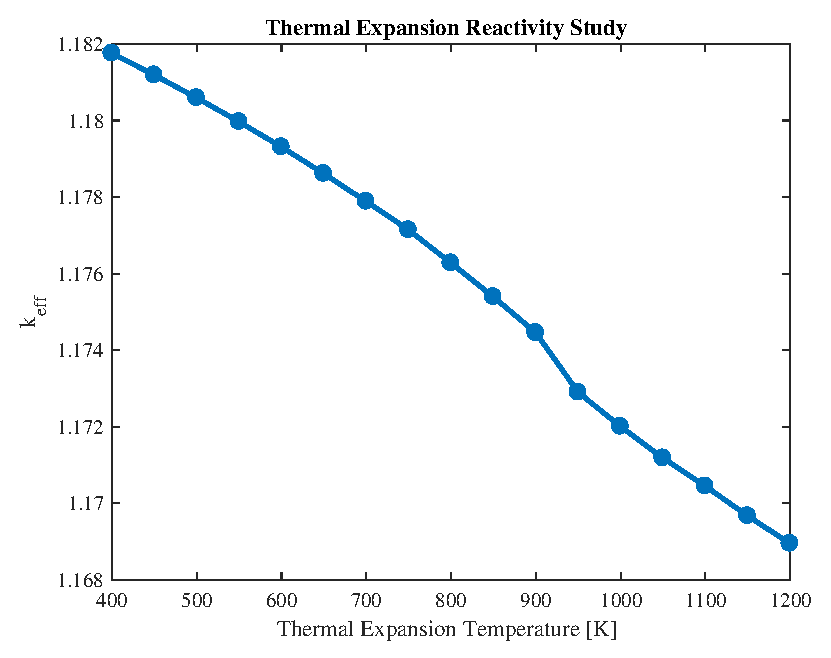
\includegraphics[width=0.7\textwidth]{thexp_study}
    \caption{Effective Neutron Multiplication Factor as a Function of 
      Thermal Expansion Temperature.}
    \label{fig:thexp_study}
  \end{figure}

  \begin{figure}
    \centering
    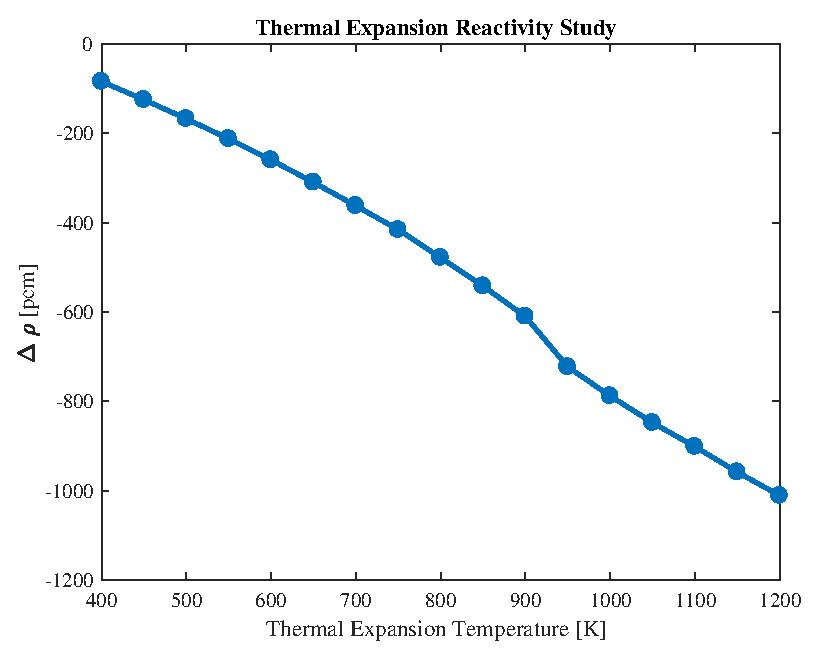
\includegraphics[width=0.7\textwidth]{thexp_study_reactivity}
    \caption{Reactivity as a Function of Thermal Expansion Temperature.}
    \label{fig:thexp_study_reactivity}
  \end{figure}

\chapter{Coupled Results}
\label{ch:coupledResults}

\section{Power Reactor Modeling}
\label{sec:power_reactor_modeling}
  The motivation for this work is to model nuclear power reactors with
  multiphysics feedback. This has been accomplished by modeling power
  distribution with the multigroup neutron diffusion equation solved via the
  Finite Element Method (FEM) (\chref{ch:neutronDiffusion}), axial heat
  convection and radial heat conduction models (\chref{ch:thermalHydraulics}),
  and simplified thermal expansion modeling (\chref{ch:thermalExpansion}).
  Combined, these effects will provide feedback which can be estimated in the
  model. 
  
  A realistic reactor benchmark is provided and modeled \sref{sec:abr}.
  Reactivity coefficients describing system responses are defined in
  \sref{sec:reactivity_coefficients}. Results are presented in
  \sref{sec:results}.

\section{Advance Burner Reactor -- MET 1000}
\label{sec:abr}
  This problem is proposed by Organisation for Economic Co-operation and
  Development Nuclear Energy Agency (OECD NEA) in \cite{abr}. The Advanced
  Burner Reactor (ABR) is fueled with a ternary metallic fuel and has a 1000
  \units{MWth} rating. This is a medium-sized metalic reactor with a total of
  180 assemblies and is 4.8 \units{m} tall. The benchmark is fully specified and
  thirty-one independent results are submitted. Each submission has generated
  its own cross-sections. Submissions include a solution using \dif.

  The materials in the benchmark are shown in \fref{fig:abr_materials}. Fast
  neutron flux is shown to peak in the core center and thermal neutron flux is
  shown to peak in the structural material surrounding the core in
  \fref{fig:abr_fluxes}.

  \begin{figure}
    \centering
    \includegraphics[width=0.3\textwidth]{abr_materials}
    \caption{Materials in ABR.}
    \label{fig:abr_materials}
  \end{figure}

  \begin{figure}
    \centering
    \subfloat[$\phi_{1}$]{
      \includegraphics[width=0.25\textwidth]{abr_phi_nod_group1}}
    \hspace{0.2in}
    \subfloat[$\phi_{33}$]{
      \includegraphics[width=0.25\textwidth]{abr_phi_nod_group33}}
    \caption{Multigroup Neutron Flux in ABR.}
    \label{fig:abr_fluxes}
  \end{figure}

\section{Reactivity Coefficients}
\label{sec:reactivity_coefficients}
  % give formulae for everything

\section{Results}
\label{sec:results}


\chapter{Discussion, Conclusions, and Recommendations}
\label{ch:conclusions}

\section{Discussion of Simulation Results}

  The purpose of this thesis is to simulate a Fast Reactor (FR) at operating
  reactor power conditions with coupled multiphysics simulations. The method
  developed allows for solution to the multigroup neutron diffusion equation for
  general unstructured mesh. The coupled multiphysics models allows for inherent
  modeling instead of thermal feedback effects instead of using extremely
  simplified and manual models. By including all simulations in a single
  simulation suite, a user can more easily observe the interaction of 
  physical phenomena and feedback.

  In \chref{ch:neutronDiffusion}, a rigorous and general framework is developed
  for solving the multigroup neutron diffusion equation using the FEM for
  general unstructured mesh. Insights are provided into the use of both
  two-dimension triangular elements and three-dimensional wedge (pentahedral)
  elements. Both of these geometries are natural choices for FRs which typically
  employ hexagonal geometries. Using the developed methods,
  \chref{ch:diffusionResults} then demonstrates solution verification and
  solution validation for both analytic and reactor benchmark problems. The
  multigroup neutron diffusion solver as implemented is shown to converge to the
  correct answer at the correct convergence rate.

  \chref{ch:thermalHydraulics} presents the details of the thermal hydraulic
  models employed. These models include an axial convection model and a radial
  conduction model. The results of the thermal hydraulic calculations are
  material temperatures that are used to interpolate cross-section tables and
  update coolant density to generate temperature-dependent cross-sections.

  In \chref{ch:thermalExpansion}, a simplified thermal expansion model is
  presented. The model expands materials linearly assuming expansion as either
  HT9 Stainless-Steel structural material or U10Zr fuel material. The model
  requires an \textit{a priori} assumption of material temperatures but results
  are not highly sensitive to these temperatures due to the magnitudes of
  thermal expansion coefficients.

  Finally, \chref{ch:coupledResults} presents the culmination of all models
  implemented. A typical FR as presented in a benchmark problem is simulated.
  Using the models developed, reactivity coefficients can be estimated for an
  operating reactor. These coefficients describe dynamic reactor behavior and
  agree with expected values. These reactivity coefficients also describe the
  mechanisms for inherent safety in a FR.

\section{Conclusions}
  
  It has been demonstrated that the FEM can be used to efficiently simulate the
  power distribution in a nuclear power reactor. Use of the FEM has allowed for 
  the local simulation of multiphysics effects within elements. By simulating
  thermal hydraulic feedback and thermal expansion effects, reactivity effects
  are estimated. Prior to this coupling method, the simulation of feedback
  effects required either manual iterative process between thermal hydraulic 
  codes and neutron diffusion codes or the use of simplified estimates of 
  temperatures. 
  
\section{Recommendations for Future Research}

  The results of this thesis demonstrate a framework for an all-in-one reactor 
  simulator for FR simulations. Future work includes code enhancements,
  added features, and simulation of new reactors. Ultimately, the goal is to
  develop a reactor simulation suite that can be used to perform core design
  calculations and analyze dynamic reactive behavior.

  \subsection{Encouraging Code Usage}
    

  \subsection{Code Enhancements}
    Depletion, Higher Order elements, \& SPN
 
  \subsection{Further Investigations}
    \begin{itemize}
      \item SuperPhenix Benchmark
      \item EBR-II modeling
    \end{itemize}


%%---------------------------------------------------------------------------%%
%%  Bibliography 
%% or use BibTeX
%Citations should be of the form ``author year''  not ``author, year''

%%%% \bibpunct{(}{)}{;}{a}{}{,} % changes apalike bst into AMS format
%%%% \bibliography{dissertation.bib}
%%%% \bibliographystyle{apalike}

\begin{singlespace}
\printbibliography[title=REFERENCES]
\addcontentsline{toc}{chapter}{References}
\end{singlespace}

%%---------------------------------------------------------------------------%%
% Appendices
%\ensureoddstart
\restoregeometry
\appendix
%\newgeometry{margin=1in,lmargin=1.25in,footskip=\chapterfootskip, includehead, includefoot}

% Can remove or add
\chapter{Analytic Solutions to the Neutron Diffusion Equation}

\section{A First Section}
\section{A Second Section}

\chapter{Brief Compendium of Neutron Diffusion Benchmarks}
\label{ap:benchmarks}

\section{Introduction}
\section{Two Dimension}
  \subsection{VVER440}
  \subsection{SNR}
  \subsection{IAEA}
\section{Three Dimension}
  \subsection{MONJU}
  \subsection{KNK}



\restoregeometry

%%---------------------------------------------------------------------------%%

%%---------------------------------------------------------------------------%%
\backmatter

\end{document}
